\documentclass[letter,8pt]{article}\usepackage[]{graphicx}\usepackage[]{color}
% maxwidth is the original width if it is less than linewidth
% otherwise use linewidth (to make sure the graphics do not exceed the margin)
\makeatletter
\def\maxwidth{ %
  \ifdim\Gin@nat@width>\linewidth
    \linewidth
  \else
    \Gin@nat@width
  \fi
}
\makeatother

\definecolor{fgcolor}{rgb}{0.345, 0.345, 0.345}
\newcommand{\hlnum}[1]{\textcolor[rgb]{0.686,0.059,0.569}{#1}}%
\newcommand{\hlstr}[1]{\textcolor[rgb]{0.192,0.494,0.8}{#1}}%
\newcommand{\hlcom}[1]{\textcolor[rgb]{0.678,0.584,0.686}{\textit{#1}}}%
\newcommand{\hlopt}[1]{\textcolor[rgb]{0,0,0}{#1}}%
\newcommand{\hlstd}[1]{\textcolor[rgb]{0.345,0.345,0.345}{#1}}%
\newcommand{\hlkwa}[1]{\textcolor[rgb]{0.161,0.373,0.58}{\textbf{#1}}}%
\newcommand{\hlkwb}[1]{\textcolor[rgb]{0.69,0.353,0.396}{#1}}%
\newcommand{\hlkwc}[1]{\textcolor[rgb]{0.333,0.667,0.333}{#1}}%
\newcommand{\hlkwd}[1]{\textcolor[rgb]{0.737,0.353,0.396}{\textbf{#1}}}%
\let\hlipl\hlkwb

\usepackage{framed}
\makeatletter
\newenvironment{kframe}{%
 \def\at@end@of@kframe{}%
 \ifinner\ifhmode%
  \def\at@end@of@kframe{\end{minipage}}%
  \begin{minipage}{\columnwidth}%
 \fi\fi%
 \def\FrameCommand##1{\hskip\@totalleftmargin \hskip-\fboxsep
 \colorbox{shadecolor}{##1}\hskip-\fboxsep
     % There is no \\@totalrightmargin, so:
     \hskip-\linewidth \hskip-\@totalleftmargin \hskip\columnwidth}%
 \MakeFramed {\advance\hsize-\width
   \@totalleftmargin\z@ \linewidth\hsize
   \@setminipage}}%
 {\par\unskip\endMakeFramed%
 \at@end@of@kframe}
\makeatother

\definecolor{shadecolor}{rgb}{.97, .97, .97}
\definecolor{messagecolor}{rgb}{0, 0, 0}
\definecolor{warningcolor}{rgb}{1, 0, 1}
\definecolor{errorcolor}{rgb}{1, 0, 0}
\newenvironment{knitrout}{}{} % an empty environment to be redefined in TeX

\usepackage{alltt} 

%%%%%%%%%%%%%%%%%%%%
%%%%%% Package %%%%%
%%%%%%%%%%%%%%%%%%%%

%\usepackage[latin1]{inputenc}
\usepackage[parfill]{parskip} % Activate to begin paragraphs with an empty line rather than an indent
\usepackage{amsmath,amsthm,amssymb,bbm} %math stuff
\usepackage{placeins} % FloatBarrier
\usepackage{fancyhdr}
\usepackage{lastpage}
\usepackage{float}    % for fig.pos='H'
%\usepackage{subfig}   % for subfigure
\usepackage{subcaption}  % an alternative package for sub figures
\usepackage{comment}
\bibliographystyle{plainnat}
\usepackage{setspace} %Spacing
\usepackage{graphicx,graphics}
\usepackage{booktabs,tabularx}
\usepackage{enumerate}
\usepackage{makecell}
\usepackage{xfrac}
\restylefloat{figure}
\usepackage{appendix}
\usepackage{color, colortbl, xcolor}
\usepackage{booktabs,dcolumn} % for use with texreg in R
\usepackage[bookmarks]{hyperref}
\usepackage[numbers]{natbib}
\bibliographystyle{ksfh_nat}
\usepackage{wrapfig}
\usepackage{todonotes}
\usepackage{fancyvrb}



%%%%%%%%%%%%%%%%%%%%%%%%%
%%%%%% Configuration %%%%
%%%%%%%%%%%%%%%%%%%%%%%%%

\newcommand{\nd}{\noindent}
\newcommand{\ntodo}[2][]{\todo[#1]{\thesubsubsection{}. #2}}

% Define the format of the report
\renewcommand{\headrulewidth}{0.0pt}
\renewcommand{\footrulewidth}{0.0pt}
\setlength{\textheight}{9.00in}
\setlength{\textwidth}{7.00in}
\setlength{\topmargin}{-0.5in}
\setlength{\evensidemargin}{-0.25in}
\setlength{\oddsidemargin}{-0.25in}
\renewcommand{\baselinestretch}{1.2}
\makeatletter
\makeatother
\lfoot{} \cfoot{ } \rfoot{{\small{\em Page \thepage \ of \pageref{LastPage}}}}

\newenvironment{conditions}
  {\par\vspace{\abovedisplayskip}\noindent\begin{tabular}{>{$}l<{$} @{${}={}$} l}}
  {\end{tabular}\par\vspace{\belowdisplayskip}}
%%%%%%%%%%%%%%%%%%%%%%%%%%%%%%%%%%%%%%%%%%%%%%%%%%%
%%%%%%%%%%%%%%%%% BEGIN        %%%%%%%%%%%%%%%%%%%%
%%%%%%%%%%%%%%%%%%%%%%%%%%%%%%%%%%%%%%%%%%%%%%%%%%%
\IfFileExists{upquote.sty}{\usepackage{upquote}}{}
\begin{document}
\pagestyle{plain}
\pagenumbering{gobble}
\begin{titlepage}
   \begin{center}
       \vspace*{1cm}
 
       \textbf{Advanced Statistical Learning\\ (MATH80619)}
 
       \vspace{0.5cm}
        Deep Learning in R \\
        \vspace{2.5cm}
        Presented to\\
        Denis Larocque \\ Aurélie Labbe
        
       \vspace{5.5cm}
        by\\
        \vspace{0.5cm}


\begin{tabular}{ll}
    Estefan Apablaza-Arancibia & (11271806) \\
    Adrien Hernandez  & (11269225)\\ 
\end{tabular}
 
       \vfill
 
       Master of Science (M. SC.)
 
       \vspace{0.8cm}
 
       
\includegraphics[width=0.4\textwidth]{figure/hec_logo.jpg}
 
       Data Science \& Business Analytics\\
       Québec, Canada\\
       \today{}
 
   \end{center}
\end{titlepage}
\newpage
\pagestyle{plain}


%%%%%%%%%%%%%%%%%%%%%%%%%%%%%%%%%%%%%%%%%%%%%%%%%%%
%%%%%%%%%%%%%%%%% INTRODUCTION %%%%%%%%%%%%%%%%%%%%
%%%%%%%%%%%%%%%%%%%%%%%%%%%%%%%%%%%%%%%%%%%%%%%%%%%
\newpage
\pagestyle{fancy}
\pagenumbering{arabic}
\section{Introduction}
These days, "deep learning" buzz word is part of multiple repositories projects and companies around the world. Most projects are build around the programming language python. That being said it will be intersting to see if this trend is viable in the R studio environment.
To start, a literature review covers the neural networks and deep learners algorithms, focusing on different types of neural networks architectures and describing for which kind tasks each neural network architecture has been designed for. Furthermore, the methodology section will try to describe briefly the workflow of deeps learning training and predictions, the dataset that could be use for different algorithms and finally some characterstic use to compare different packages. Then, an exhaustive list of the R libraries allowing to build neural networks and deep learners models. Correspondingly, the advantages and disadvantages of each libraries, their capabilities as well as what you can expect when using them. To sum up, the last section will give concrete examples on how to implement the neural networks and deep learners models with these libraries, using the example data of the methodology section.

%%%%%%%%%%%%%%%%%%%%%%%%%%%%%%%%%%%%%%%%%%%%%%%%%%%
%%%%%%%%%%%%%%%%%% Litterature %%%%%%%%%%%%%%%%%%%%
%%%%%%%%%%%%%%%%%% Review      %%%%%%%%%%%%%%%%%%%%
%%%%%%%%%%%%%%%%%%%%%%%%%%%%%%%%%%%%%%%%%%%%%%%%%%%

\section{Litterature Review}
\subsection{What is Deep Learning and why use it?}
\begin{wrapfigure}[11]{r}{0.5\textwidth}
  \begin{center}
    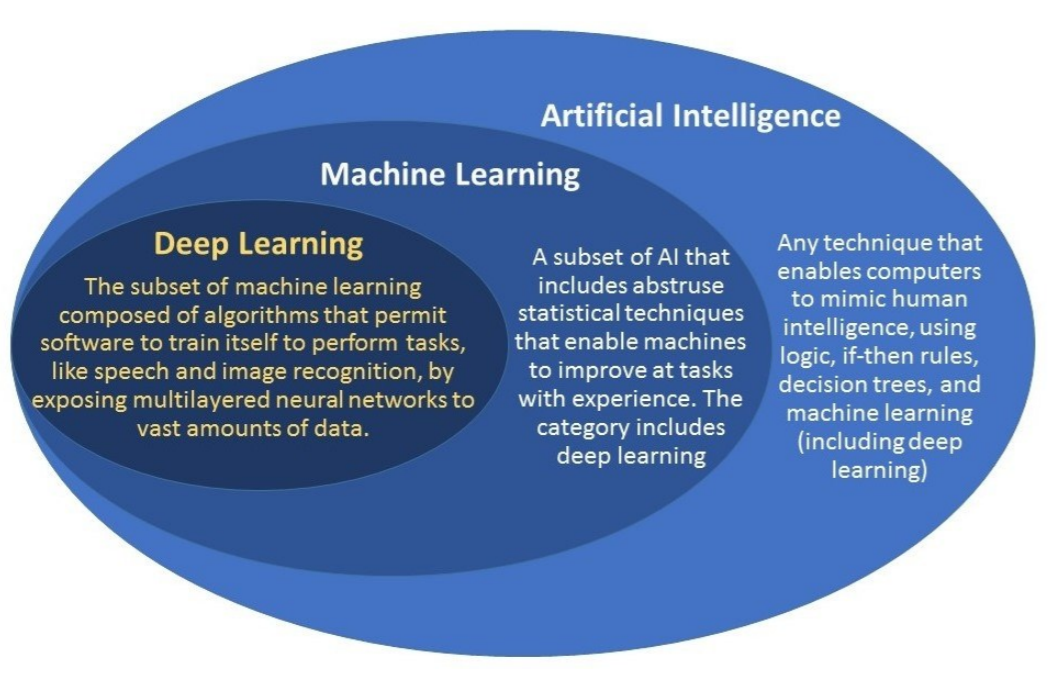
\includegraphics[width=0.4\textwidth]{figure/deep learning.PNG}
      \end{center}
     \caption{Artificial Intelligence vs Machine Learning vs Deep Learning \cite{aivsdeepvsml}}
     \label{fig:simule}
\end{wrapfigure}

Deep learning is a subset field of articial intelligence and can be seen as a specific way of doing machine learning. Deep learning algorithms can be seen as feature representation learning. Indeed, by applying to the data multiple non-linear transformations through the use of hidden layers, deep learning models have their own trainable feature extration capability making it possible to learn specific features from the data without needing a specific human domain expert. This means that deep learning models won't require the features extraction step that is essential for classic machine learning models. However, increasing the models capacity by adding hidden layers, requires increasingly computing power and slow down the training process of the model. The choice of hyperparameters, programming languages and memory management will therefore be important criteria to take into account while building deep learning models\\
Since the last decade, deep learning models have shown notable predictive power and have been revolutionizing an important number of domain such as computer vision, natural language understanding, fraud detection, health and much more.\\
As a first glance in the subject, it is highly recommended it to read  a reference from pioneers in the field (\cite[Chapter 1]{Goodfellow-et-al-2016}).


\subsubsection{Feed Forward Neural Network}
\begin{wrapfigure}[11]{R}{0.5\textwidth}
  \begin{center}
    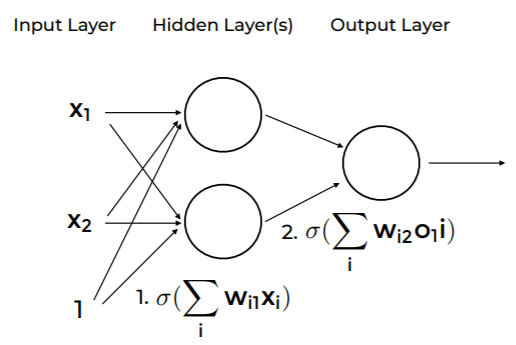
\includegraphics[width=0.4\textwidth]{figure/feedforward_neural_networks.png}
  \end{center}
  \caption{feedforward neural networks}
  \label{fig:attention}
\end{wrapfigure}

"Deep feedforward networks, also called feedforward neural networks, or multilayer perceptrons (MLPs), are the quintessential deep learning models." \cite{Goodfellow-et-al-2016}

FNN models are inspired from biology and by the way the human brain works. In a neural network, each neuron takes input from other neurons, processes the information and then transmits outputs to next neurons. Artificial neural networks follow the same process as each neuron will perform the weighted sum of inputs and will add a bias as a degree of freedom. It will then apply a non-linear transformation before outputting the information. Thus, the information goes forward in the network; neurons transmit information from the input layers towards the output layer. It is important to know that in a feedfoward neural networks (fig. \ref{fig:attention}) the neurons of a same layer are not connected to each other; they do not allow any feedback connections within a same layer. If we want to allow this process, we will be looking at recurrent neural networks.

The equation a neuron input is  
\begin{equation}
a(x) = b +\sum_{i}{w_i x_i}
\end{equation}
and the output
\begin{equation}
h(x) = g(a(x))
\end{equation}
where:
\begin{conditions}
 x     &  the input data \\
 b     &  the bias term \\
 w     &  the weight or parameter \\   
 g(...) &  the activation function
\end{conditions}

\begin{wrapfigure}[13]{r}{0.5\textwidth}
  \begin{center}
    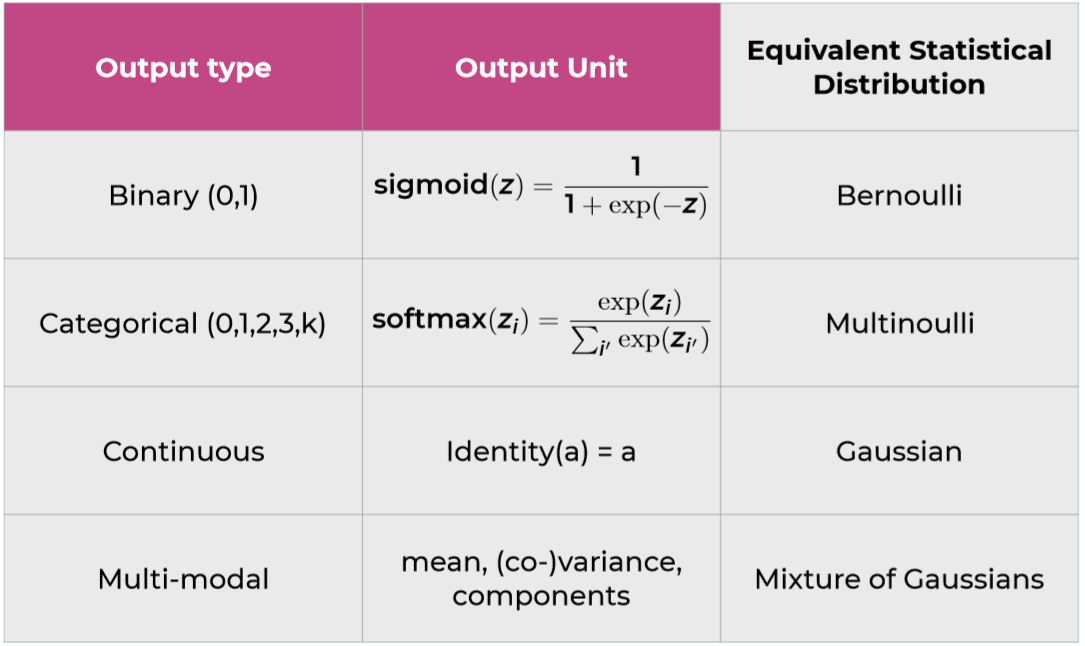
\includegraphics[width=0.45\textwidth]{figure/activation_function_output.png}
      \end{center}
     \caption{Activation functions: output units. \cite[slide 24]{nnheca2019}}
     \label{fig:activation}
\end{wrapfigure}
Here, \textbf{the bias term  b} and \textbf{the weights or parameter w} will be learned by the model in order the minimize a cost function, through the use of the gradient descent method. Then, the network will use the backpropagation algorithm where the error is backpropagated from the output to the input layers and the bias and weighted are then updated accordingly.\\
Regarding the \textbf{activation function g(...)}, the common practice is to use a ReLu (rectified linear unit) as the activation function for the neurons of the hidden layers. Regarding the neurons of the last layer, the activation function will be chosen accordingly to the task we want our model to perform:



A detailed explanation of the theory of feedforward neural network can be found in \cite[Chapter 6]{Goodfellow-et-al-2016}

\subsubsection{CNN}

The CNN are a modified architecture of FNN that leverage the feature engineering that used to be hand maded by domain experts. This class of deep neural network are commonly used for image recognition and classification that can serve different applications such as facial recongnition, document analysis and speech recognition. The original FNN are not suited analyzing large size images since the weights increase exponentially and, at the end, don't perfom very well.\\
\begin{wrapfigure}[8]{r}{0.5\textwidth}
  \begin{center}
    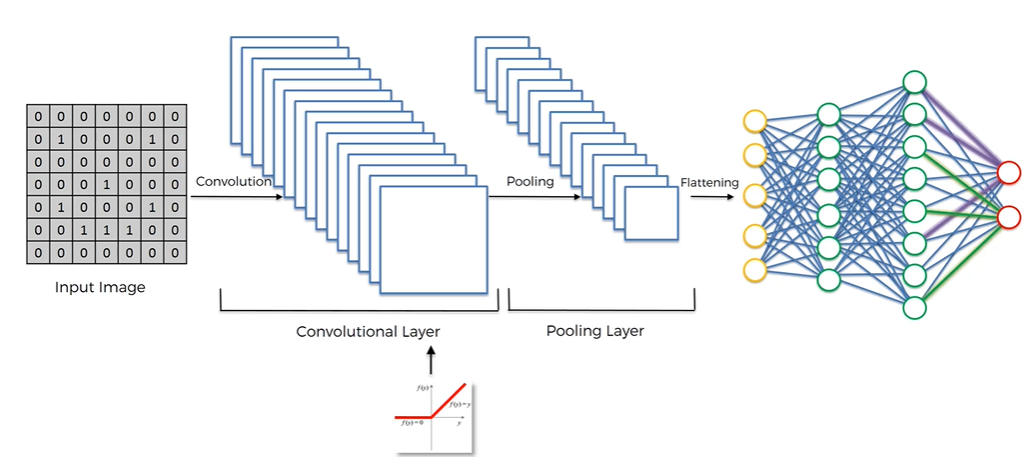
\includegraphics[width=0.5\textwidth]{figure/CNN_process.png}
  \end{center}
  \caption{CNN, Deep Learning A-Z by SuperDataScience}
\end{wrapfigure}
A standard architecture of a CNN model is commonly represented this way:
\begin{itemize}
\item We start with an input image to which we are going to apply several kernels, a.k.a features detectors, in order to create feature maps that will form what we call a convolutional layer. 
\item A common practice is to apply the ReLu activation fonction to the convolutional layer output in order to increase the non linearity of the images.
\item Then we use the pooling method to create a pooling layer.
\item The next step will be to combine all the pooled images from the pooling layer into one single vector, which is called flattening and will be the input of a FNN that will perform the desired task, for instance, classification. 
\end{itemize}
CNN parameters are trained with the \textbf{backpropagation} algorithm where the gradients are propagated from the output layer of the FFN to the input of the CNN in order to minimise a cost function, most of the time a categorical cross-entropy if we are performing a multi-class classification. 


To get a detailed explanation of convolutional neural networks we recommand to read \cite[Chapter 9]{Goodfellow-et-al-2016}.\\

\subsubsection{RNN}
Recurrent neural networks are a more advanced type of deep learning architecture having proven state-of-art performance for solving tasks related to sequential data such as Natural Language Processing (NLP), anomaly detection and event forecasting. As a key differentiator from feedfoward neural networks, is that RNNs use feedback loops connections instead of feedforward connections and get an internal memory. Indeed, that take as input each step of the sequantial data as well as what they have learned over time. One of their other advantage is to be able to handle input and ouput sequences with different sizes. "A recurrent neural network can be thought of as multiple copies of the same network, each passing a message to a successor" Olah.
\begin{wrapfigure}[12]{r}{0.5\textwidth}
    \begin{center}
    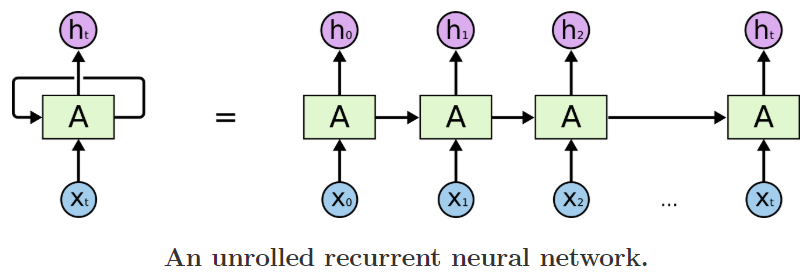
\includegraphics[width=0.45\textwidth]{figure/RNN_process.png}
    \end{center}
     \caption{RNN, Understanding LSTM Networks by Olah}
     \label{fig:rnn_process}
\end{wrapfigure}

A standard architecture of a RNN model is commonly
represented this way:
\begin{itemize}
\item The training uses the input \textit{x} as part of the data sequence or vector. For example, if our data is \textbf{x = "I am learning deep learning"}, then our $x_1$ will be "I", and our $x_2$ will be "am", etc.
\item We will also use a second input which is the hidden state of the previous cell of our network. This means that in this network our neurons are connected by a feedback loop. This will allow our network to capture the "temporal" information of our data and gives it a memory. 
\end{itemize}

RNN parameters are trained with the \textbf{backpropagation through time} algorithm where the gradients are propagated from the output layer of the RNN in order to minimise a cost function, most of the time a categorical cross-entropy if we are performing a multi-class classification for example. However, a simple RNN network will suffer of gradient vanishing or exploding because the sequence lengths. State-of-art algorithms such as GRU or LSTM exists to tackle this problem.  

A detailed explanation of recurrent neural networks can be found in the  \cite[Chapter 10]{Goodfellow-et-al-2016}. We also recommand reading this blog post \cite{olah_2015}.

\subsection{Deep Learning integration in R}
\label{sec:deepinR}
The integration of Deep learning in R can be separate in two part ; (1) The API integration and (2) the standalone R packages. 
\begin{enumerate}
\item The API will give the possibility to control externally through R an existing installation. In other words, a software translator for a already known software installation. This approach is not always trivial to install nor to manipulate but in long term will probably give the best flexibility in terms of Deep Learning projects.
\item The standalone R packages will be packages that require no third party software in order to create the deep learning projects. This approach is relatively fast to install but is restraing in terms deep learning architecture.
\end{enumerate}
A list of the available resources with installation and examples tutorials can be found in section \ref{avail_ressour} and \ref{examples} .

%%%%%%%%%%%%%%%%%%%%%%%%%%%%%%%%%%%%%%%%%%%%%%%%%%%
%%%%%%%%%%%%%%%%%% Description %%%%%%%%%%%%%%%%%%%%
%%%%%%%%%%%%%%%%%% of methods  %%%%%%%%%%%%%%%%%%%%
%%%%%%%%%%%%%%%%%%%%%%%%%%%%%%%%%%%%%%%%%%%%%%%%%%%
\section{Methodology}
This section is divided in two;  the dataset description and the benchmark type. The dataset description is mostly to describe what dataset is going to be use for the different type of deep learning algorithms. The second section will describe two indicators in order to compare results of similar algorithms. The first indicator is mostly about a simple accuracy base on the same training and validation dataset and second indicator is about the time it took to execute the same task on differents ressources.
\subsection{Workflow}
The workflow of a deep learning project in R we recommand to follow is described below:
\begin{itemize}
\item Collection, pre-processing and cleaning of the data in order to make them ready to train the model. Partition the data into a training set and a validation/test set (Most of the time 80\% of the data goes to training and 20\% goes to testing). You can use cross-valiation if you don't have enough data, but it shouldn't be the case in most of the deep learning projects.
\item Choose the right model according to the task you want to perform. Some models have been especially created in order to perform well on a specific task, for example, CNN have been created to solve images classification related tasks.
\item Train the selected models with your training data by checking at the same time how your validation accuracy (or another metric that corresponds the best to your task) is evolving through the training process.
\item Modify your models' hyperparameters and experiment changes in the model architecture in order to improve your model accuracy.
\item Evaluate and compare your models on the test data.
\end{itemize}
\subsection{Dataset}
\subsubsection{FNN}
For the FNN, the training data will be the well known \textit{Iris} dataset. It contains four covariables (Length and Width of Sepal and Petals) and one categorical target variable representing 3 type iris species ((\textit{Iris setosa}, \textit{Iris virginica} and \textit{Iris versicolor})).  This dataset of 50 observations is pretty well known and is perfect to show a small example of FNN. 

\subsubsection{CNN}
For the CNN, the training data will also be a well known dataset called CIFAR-10. The CIFAR-10 dataset consists of 60000 32x32 colour images in 10 classes, with 6000 images per class. The easiest way in R to download this package is using the Keras API. The training dataset has 50 000 images in three color (Red-Green-Blue) that are 32 pixels by 32 pixels. The testing dataset has a total of 10 000 images

\subsubsection{RNN}
The dataset use to test an RNN is the IMDB Movie reviews for sentiment classification. The reason to use this dataset is that Keras API also offers a complete bundle (of 25 000 reviews for training and another 25 000 for testing) with multiple parameter to help you get started with sentimen classification using RNN. Each review is classify as "1" (good) or "0" (bad) and the word index is already done. The total word vocabulary is 88 000 words.



\subsection{Characteristic}
\subsubsection{Accuracy}
As the purpose of this tutorial is to learn to build the architecture of neural networks in R, we will not focus on accuracy measurement.However, it might come handy for users to have a tool or starting point therefore an extensive readin of this source \cite{perfomancelink} is highly recommend.
Since for all three algorithms (FNN , CNN and RNN) it is mostly a classification models the accuracy will be $1-classification_{error}$.
\subsubsection{Time elapsed}
Sometime the training timing can be a deal breaker for some users. This charactersitic is calculated from a simple R package ,that being said it is really important to not generalised the tutorials results. It is simply to give an idea about the training time since it depends on multiple factor (e.g. Computer characterstics such as memory , CPU, etc.).


%%%%%%%%%%%%%%%%%%%%%%%%%%%%%%%%%%%%%%%%%%%%%%%%%%%
%%%%%%%%%%%%%%%%%% Resources   %%%%%%%%%%%%%%%%%%%%
%%%%%%%%%%%%%%%%%% available   %%%%%%%%%%%%%%%%%%%%
%%%%%%%%%%%%%%%%%%%%%%%%%%%%%%%%%%%%%%%%%%%%%%%%%%%

\section{Available resources}
\label{sec:avail_ressour}
As mentioned in the section \ref{sec:deepinR}, we will firstly introduce the most important R packages coming from the CRAN platform for deep learning. Then, we will give an overview of the different API packages available. For each R package (not API based), we give a description as well as a visual example of how to build a neural network model with it. Moreover, we highlight the most important Pros and Cons, although we highly suggest you to read the packages official documentation that we also provide.
%%%%%%%%%%%%%%%%%%%%%%%%%%%%%%%%%%%%%%%%%%%%%%%%%%%
%%%%%%%%%%%%%%%%%% R Packages   %%%%%%%%%%%%%%%%%%%%
%%%%%%%%%%%%%%%%%%%%%%%%%%%%%%%%%%%%%%%%%%%%%%%%%%%
\subsection{R packages}


%%%%%%%%%%%%%%%% Neuralnet %%%%%%%%%%%%%%%% 
\subsubsection{\textbf{Neuralnet package}}
\paragraph{Description}
According to its CRAN description, the package allows the "training of neural networks using the backpropagation, resilient backpropagation with (Riedmiller, 1994) or without weight backtracking (Riedmiller, 1993) or the modified globally convergent version by Anastasiadis et al. (2005). The package allows flexible settings through custom-choice of error and activation function. Furthermore, the calculation of generalized weights (Intrator O \& Intrator N, 1993) is implemented." This package uses $C/C++$ in backend. More information can be found on the package source \cite{neuralnet2019}.

\textit{Important default parameters of a FNN model with the neuralnet package:}
\begin{figure}[H]
  \begin{subfigure}{0.5\textwidth}
\begin{knitrout}
\definecolor{shadecolor}{rgb}{0.969, 0.969, 0.969}\color{fgcolor}\begin{kframe}
\begin{alltt}
\hlkwd{neuralnet}\hlstd{(formula,}
      \hlkwc{data} \hlstd{= Y}\hlopt{~}\hlstd{X1}\hlopt{+}\hlstd{...}\hlopt{+}\hlstd{Xn,}
      \hlkwc{hidden} \hlstd{=} \hlnum{1}\hlstd{,}
      \hlkwc{threshold} \hlstd{=} \hlnum{0.01}\hlstd{,}
      \hlkwc{stepmax} \hlstd{=} \hlnum{1e+05}\hlstd{,}
      \hlkwc{rep} \hlstd{=} \hlnum{1}\hlstd{,}
      \hlkwc{startweights} \hlstd{=} \hlkwa{NULL}\hlstd{,}
      \hlkwc{learningrate.limit} \hlstd{=} \hlkwa{NULL}\hlstd{,}
      \hlkwc{algorithm} \hlstd{=} \hlstr{"rprop+"}\hlstd{,}
      \hlkwc{err.fct} \hlstd{=} \hlstr{"sse"}\hlstd{,}
      \hlkwc{act.fct} \hlstd{=} \hlstr{"logistic"}\hlstd{,}
      \hlkwc{linear.output} \hlstd{=} \hlnum{TRUE}\hlstd{)}
\end{alltt}
\end{kframe}
\end{knitrout}
    \caption{Training function}
  \end{subfigure}
  \begin{subfigure}{0.5\textwidth}
    \centering
\begin{knitrout}
\definecolor{shadecolor}{rgb}{0.969, 0.969, 0.969}\color{fgcolor}\begin{kframe}
\begin{alltt}
\hlcom{#' @param formula : a symbolic description of }
\hlcom{#         the model to be fitted.}
\hlcom{#' @param data : a data frame containing the }
\hlcom{#         variables specified in formula.}
\hlcom{#' @param hidden : a vector of integers }
\hlcom{#         specifying the number of hidden }
\hlcom{#         neurons (vertices) in each layer.}
\hlcom{#' @param threshold : a numeric valuethe }
\hlcom{#         threshold for the partial }
\hlcom{#         derivatives of the error function }
\hlcom{#         as stopping criteria.}
\hlcom{#' @param stepmax : the maximum steps for }
\hlcom{#         the training of the neural network.}
\hlcom{#' @param rep : the number of repetitions }
\hlcom{#         for the neural network’s training.}
\hlcom{#' @param algorithm : a string containing }
\hlcom{#         the algorithm type to calculate the }
\hlcom{#         neural network.}
\hlcom{#' @param err.fct : a differentiable function }
\hlcom{#         that is used for the calculation of }
\hlcom{#         the error}
\hlcom{#' @param act.fct : a differentiable function }
\hlcom{#         that is #used for smoothing the result }
\hlcom{#         of the cross product of the covariate }
\hlcom{#         or neurons and the weights.}
\hlcom{#' @param linear.output :  If act.fct should not}
\hlcom{#         be applied to the output neurons set }
\hlcom{#         linear output to TRUE, otherwise to FALSE.}
\hlcom{#' @return a neuralnet model}
\end{alltt}
\end{kframe}
\end{knitrout}
    \caption{Parameters}
  \end{subfigure}
    \caption{Neuralnet package}
\end{figure}


\paragraph{Pros}
\begin{itemize}
\item Very easy to use and to build a quick FFN and deep FNN model.
\item Allows to use several types of backpropagation algorithms. By default, the resilient backpropagation algorithm is used "rprop+" instead of regular backpropagation which is an algorithm not very used in practice as it is more tricky to implement. We can however decided to change the rprop+ for a standard backpropagation by changing for \textbf{algorithm = "backprop"}.
\item Several hidden layers and neurons per layer can be added. By default, the algorithm uses only 1 hidden layer with 1 neuron, but it can be increased by addind the command line: \textbf{hidden = c(3,3)} to get 2 hidden layers of 3 neurons each.
\item Allows to easily plot and visualize the model and its parameters with the command line: \textbf{plot(model).}
\item Allows to use custome activation functions.
\end{itemize}
\paragraph{Cons}
\begin{itemize}
\item One of the disadvantage of this package is that it requires some data preprocessing as it only works with numeric inputs. Therefore, factor variables will need to be transformed into dummies during the preprocessing phase. 
\item The package doesn't provide built-in normalization functions. Therefore, it is recommended to manually normalize the data before using them as input in the neural networks in order to reduce the number of iretation of the algorithm.
\end{itemize}

%%%%%%%%%%%%%%%% nnet %%%%%%%%%%%%%%%% 
\subsubsection{\textbf{nnet package}}
\paragraph{Description}
This package comes from the CRAN platform and allows to build and fit "FNN with a single hidden layer and multinomial log-linear models". This package uses C/C++ in backend. More information can be found on the package source \cite{nnet2020}.

\textit{Important default parameters of a FNN model with the neuralnet package:}
\begin{figure}[H]
  \begin{subfigure}{0.5\textwidth}
\begin{knitrout}
\definecolor{shadecolor}{rgb}{0.969, 0.969, 0.969}\color{fgcolor}\begin{kframe}
\begin{alltt}
\hlkwd{nnet}\hlstd{(X, Y,}
     \hlstd{size,}
     \hlkwc{linout}\hlstd{=}\hlnum{FALSE}\hlstd{,}
     \hlkwc{entropy}\hlstd{=}\hlnum{FALSE}\hlstd{,}
     \hlkwc{softmax}\hlstd{=}\hlnum{FALSE}\hlstd{,}
     \hlkwc{maxit} \hlstd{=} \hlnum{100}\hlstd{,}
     \hlkwc{decay} \hlstd{=} \hlnum{0}\hlstd{)}
\end{alltt}
\end{kframe}
\end{knitrout}
    \caption{Training function}
  \end{subfigure}
  \begin{subfigure}{0.5\textwidth}
    \centering
\begin{knitrout}
\definecolor{shadecolor}{rgb}{0.969, 0.969, 0.969}\color{fgcolor}\begin{kframe}
\begin{alltt}
  \hlcom{#' @param X : x values for examples}
  \hlcom{#' @param Y : target values for examples}
  \hlcom{#' @param size : number of units in the hidden }
  \hlcom{#         layer}
  \hlcom{#' @param linout : switch for linear output }
  \hlcom{#         units}
  \hlcom{#' @param entropy : switch for entropy}
  \hlcom{#' @param softmax : switch for softmax}
  \hlcom{#' @param maxit : maximum number of iterations}
  \hlcom{#' @param decay : parameter for weight decay}
  \hlcom{#' @return a nnet model}
\end{alltt}
\end{kframe}
\end{knitrout}
    \caption{Parameters}
  \end{subfigure}
    \caption{nnet package}
\end{figure}


\paragraph{Pros}
\begin{itemize}
\item One of the easiest R package to build a quick FFN model.
\end{itemize}
\paragraph{Cons}
\begin{itemize}
\item It does not offer a lot of flexibility, and can only apply logistic sifmoid function for the hidden layer activation and cannot use tanH and ReLu.
\item This package does not allow to use more that one hidden layer, and does not have any feature to find the optimal number of neurones in the hidden layer. It is up to the analyst to build a loop to test by cross-validation, for exemple, the optimal hyperparameter values.
\item Cannot use classical backpropagation algorithm to train the network. It only uses the BFGS (Broyden-Fletcher-Goldfarb-Shanno) which is a Quasi-Newton method and therefore increases the number of computation to reach a local optima. However, applied on a small dataset with a model having only one hidden layer does not seem to be a problem.
\item Does not have any function to plot the model.
\end{itemize}

%%%%%%%%%%%%%%%% NeuralNetTools %%%%%%%%%%%%%%%% 

\subsubsection{\textbf{NeuralNetTools package}}
\paragraph{Description}
This package is a complement to R's neural networks packages as it allows to visualize and perform analysis on neural network models. "Functions are available for plooting, quantifying variable importance, conducting a sensitivity analysis, and obtaining a simple list of model weights." More information can be found on the package source \cite{NeuralNetTools2018}.


\begin{figure}[H]
  \begin{subfigure}{0.5\textwidth}
    \centering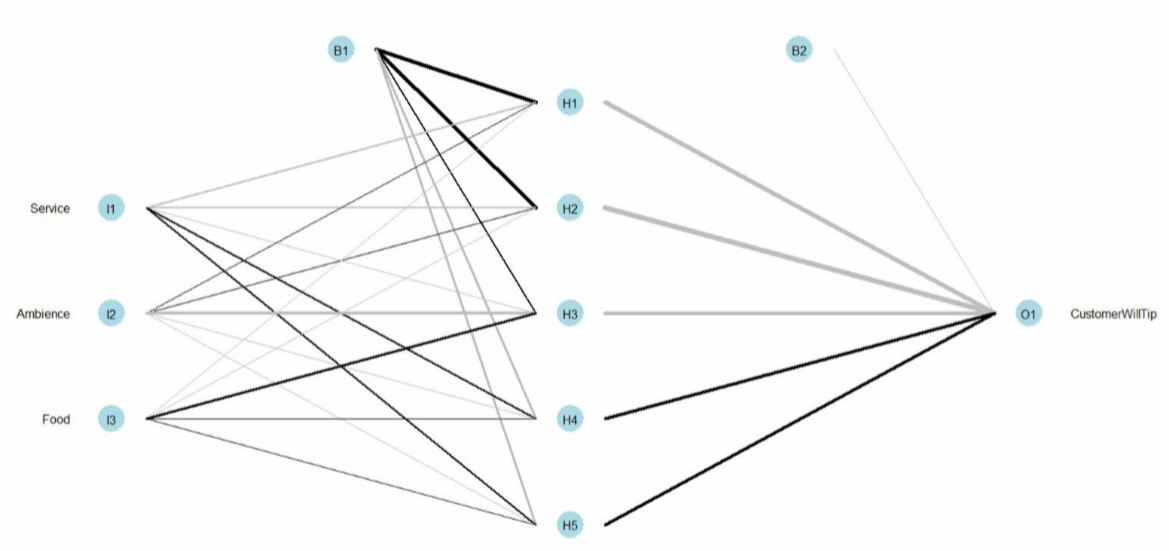
\includegraphics[width=0.45\textwidth]{figure/plotnet.png}
    \caption{NeuralNetTools, plotnet function}
  \end{subfigure}
  \begin{subfigure}{0.5\textwidth}
    \centering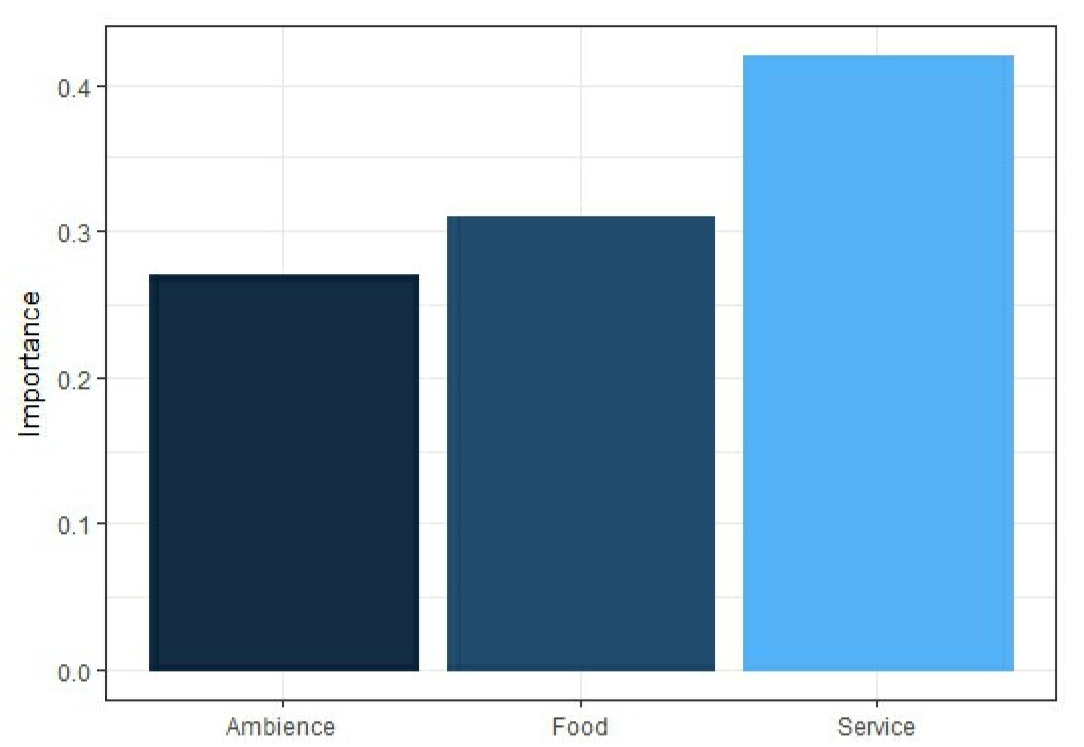
\includegraphics[width=0.45\textwidth]{figure/garson_algorithm.png}
    \caption{NeuralNetTools, Input variables importance}
  \end{subfigure}
    \caption{Embedding dimension hyper parameter \cite{Ciaburro2017NeuralNW}}
\end{figure}

\paragraph{Pros}
\begin{itemize}
\item Very easy to plot your neural network models with the function \textbf{plotnet(model)}.
\item Visualize the input variables importance to the output prediction witht the Garson and olden algorithm.
\item Perform sensitivity analysis on your neural networks model using the Lek profile method.
\item Works with the models built from different packages: \textbf{caret, neuralnet, nnet, RSNSS}
\item Can plot neural networks with pruned connections from the RSNSS package.
\end{itemize}

\paragraph{Cons}
\begin{itemize}
\item Does not provide any function for neural network model development.
\item Is not optimized to visualize large neural networks models.
\end{itemize}

%%%%%%%%%%%%%%%% Deepnet %%%%%%%%%%%%%%%% 
\subsubsection{Deepnet package}
\paragraph{Description}
This package is available on the CRAN platform and has been written specifcally written for R. It allows to "implement some deep learning architectures and neural network algorithms, including backpropagation, Restricted Boltzmann Machine (RBM), Deep Belief Network (DBN) and Deep autoencoder". More information can be found on the package source \cite{deepnet2015}.\\
\textit{Important default parameters of a deep FNN model with weights initialized by DBN:}
\begin{figure}[H]
  \begin{subfigure}{0.5\textwidth}
\begin{knitrout}
\definecolor{shadecolor}{rgb}{0.969, 0.969, 0.969}\color{fgcolor}\begin{kframe}
\begin{alltt}
\hlkwd{dbn.dnn.train}\hlstd{(X, Y,} \hlkwc{hidden}\hlstd{=}\hlkwd{c}\hlstd{(}\hlnum{5}\hlstd{),}
              \hlkwc{activationfun}\hlstd{=}\hlstr{"sigm"}\hlstd{,}
              \hlkwc{learningrate}\hlstd{=}\hlnum{0.5}\hlstd{,}
              \hlkwc{momentum}\hlstd{=}\hlnum{0.5}\hlstd{,}
              \hlkwc{learningrate_scale}\hlstd{=}\hlnum{1}\hlstd{,}
              \hlkwc{output}\hlstd{=}\hlstr{"softmax"}\hlstd{,}
              \hlkwc{numepochs} \hlstd{=} \hlnum{3}\hlstd{,}
              \hlkwc{batchsize} \hlstd{=} \hlnum{100}\hlstd{,}
              \hlkwc{hidden_dropout} \hlstd{=} \hlnum{0}\hlstd{,}
              \hlkwc{visible_dropout} \hlstd{=} \hlnum{0}\hlstd{,}
              \hlstd{)}
\end{alltt}
\end{kframe}
\end{knitrout}
    \caption{Training function}
  \end{subfigure}
  \begin{subfigure}{0.5\textwidth}
    \centering
\begin{knitrout}
\definecolor{shadecolor}{rgb}{0.969, 0.969, 0.969}\color{fgcolor}\begin{kframe}
\begin{alltt}
\hlcom{#' @param X : matrix of x values for examples}
\hlcom{#' @param Y : vector or matrix of target values }
\hlcom{#         for examples}
\hlcom{#' @param hidden : vector for number of units }
\hlcom{#         of hidden layers}
\hlcom{#' @param activationfun : activation function }
\hlcom{#         of hidden unit }
\hlcom{#' @param learningrate : learning rate for }
\hlcom{#         gradient descent}
\hlcom{#' @param momentum : momentum for gradient descent}
\hlcom{#' @param learningrate_scale :learning rate will be          #         mutiplied after every iteration}
\hlcom{#' @param output : function of output unit, can be}
\hlcom{#         "sigm","linear" or "softmax".}
\hlcom{#' @param numepochs : number of iteration }
\hlcom{#         for samples}
\hlcom{#' @param batchsize : size of mini-batch}
\hlcom{#' @param hidden_dropout : drop out fraction for}
\hlcom{#         hidden layer}
\hlcom{#' @param visible_dropout : drop out fraction }
\hlcom{#         for input layer}
\hlcom{#' @return a dbn model}
\end{alltt}
\end{kframe}
\end{knitrout}
    \caption{Parameters}
  \end{subfigure}
    \caption{Deepnet}
\end{figure}

\paragraph{Pros}
\begin{itemize}
\item Allows to load benchmark datasets such as MNIST with the function load.mnist(dir)
\item Allows to initialize the weights of a FNN with the Deep Belief Network algorithm (dbn.dnn.train()) or Stacked AutoEncoder algorithm (sae.dnn.train()).
\item Allows to have an estimation of the probabilistic distribution of a dataset trough the use of the Restricted Boltzmann machine algorithm.
\item Have more activation functions than the other R packages. Hidden Layers activation function can be linear, sigmoid or tanh. The output activation function can be linar, sigmoid or softmax.
\end{itemize}
\paragraph{Cons}
\begin{itemize}
\item Does not support the ReLu activation function for hidden layers.
\item Not the fastest package due to its implementation in R.
\item Does not provide a lot of hyperparameters tuning options, and is not user-friendly.
\end{itemize}

%%%%%%%%%%%%%%%% brnn %%%%%%%%%%%%%%%% 
\subsubsection{brnn package}
\paragraph{Description}
This package available on the platform CRAN, allows to perform "Baeysian regularized neural networks inclusing both additive and dominance effects, and allows to takes advantage of multicore architectures via a parallel computing approach using openMP for the computations" \cite{brnnarticle} therefore the package is written in R but uses the API OpenMP for faster calculation. More information can be found on the package source \cite{brnn2020}\\
\textit{Important default parameters of the brnn function:}
\begin{figure}[H]
  \begin{subfigure}{0.5\textwidth}
\begin{knitrout}
\definecolor{shadecolor}{rgb}{0.969, 0.969, 0.969}\color{fgcolor}\begin{kframe}
\begin{alltt}
\hlkwd{brnn}\hlstd{(}\hlkwc{formula}\hlstd{=  y} \hlopt{~} \hlstd{x1} \hlopt{+} \hlstd{x2,}
      \hlkwc{neurons}\hlstd{=}\hlnum{2}\hlstd{,}
      \hlkwc{normalize}\hlstd{=}\hlnum{TRUE}\hlstd{,}
      \hlkwc{epochs}\hlstd{=}\hlnum{1000}\hlstd{,}
      \hlkwc{mu}\hlstd{=}\hlnum{0.005}\hlstd{,}
      \hlkwc{mu_dec}\hlstd{=}\hlnum{0.1}\hlstd{,}
      \hlkwc{mu_inc}\hlstd{=}\hlnum{10}\hlstd{,}
      \hlkwc{mu_max}\hlstd{=}\hlnum{1e10}\hlstd{,}
      \hlkwc{min_grad}\hlstd{=}\hlnum{1e-10}\hlstd{,}
      \hlkwc{change} \hlstd{=} \hlnum{0.001}\hlstd{,}
      \hlkwc{cores}\hlstd{=}\hlnum{1}\hlstd{,}
      \hlkwc{verbose}\hlstd{=}\hlnum{FALSE}
     \hlstd{)}
\end{alltt}
\end{kframe}
\end{knitrout}
    \caption{Training function}
  \end{subfigure}
  \begin{subfigure}{0.5\textwidth}
    \centering
\begin{knitrout}
\definecolor{shadecolor}{rgb}{0.969, 0.969, 0.969}\color{fgcolor}\begin{kframe}
\begin{alltt}
\hlcom{#' @param formula : A formula of the form }
\hlcom{#         y ~ x1 + x2}
\hlcom{#' @param neurons : the number of neurons}
\hlcom{#' @param normalize : normalize inputs and output}
\hlcom{#' @param epochs : maximum number of epochs}
\hlcom{#' @param mu : positive number that controls }
\hlcom{#         the behaviour of the Gauss-Newton}
\hlcom{#         optimization}
\hlcom{#' @param mu_dec : the mu decrease ratio}
\hlcom{#' @param mu_inc : the mu increase ratio}
\hlcom{#' @param mu_max : maximum mu before training }
\hlcom{#         is stopped}
\hlcom{#' @param min_grad : minimum gradient}
\hlcom{#' @param change : The program will stop}
\hlcom{#         if the maximum}
\hlcom{#' @param cores : Number of cpu cores to}
\hlcom{#         use for calculations}
\hlcom{#' @param verbose : print iteration history}
\hlcom{#' @return a brnn model}
\end{alltt}
\end{kframe}
\end{knitrout}
    \caption{Parameters}
  \end{subfigure}
    \caption{nnet package}
\end{figure}


\paragraph{Pros}
\begin{itemize}
\item Allows to add Additive and Dominance effects in the neural networks models.
\item Take advantage of multicore processors (only for UNIX-like systems).
\item Allows to use a Gauss-Newton algorithm for optimization.
\item The package is able to assign initial weights by using the Nguyen and Widrow algorithm.
\item Include an algorithm to deal with ordinal data by using the function \textbf{brnn\_ordinal(x, ...)}
\item It has a function to normalize and unnormalized the data.
\end{itemize}
\paragraph{Cons}
\begin{itemize}
\item Cannot use the classic backpropagation algorithm for optimization.
\item The package fits a two layers neural networks and it is not possible to increase the number of hidden layers.
\end{itemize}

%%%%%%%%%%%%%%%% rnn %%%%%%%%%%%%%%%% 
\subsubsection{rnn package}
\paragraph{Description}
Avaible from the CRAN platform, this package allows the "implementation of a Recurrent Neural Network architectures in native R, including Long-Short Term Memory (LSTM), Gated Recurrent Unit (GRU) and vanilla RNN." More information can be found on the package source \cite{rnn2019}

\textit{Important default parameters of the rnn function:}

\begin{figure}[H]
  \begin{subfigure}{0.5\textwidth}
\begin{knitrout}
\definecolor{shadecolor}{rgb}{0.969, 0.969, 0.969}\color{fgcolor}\begin{kframe}
\begin{alltt}
\hlcom{# train the model}
\hlstd{model} \hlkwb{<-} \hlkwd{trainr}\hlstd{(}\hlkwc{Y}\hlstd{=data_y,}
                \hlkwc{X}\hlstd{=data_x,}
                \hlkwc{learningrate} \hlstd{=} \hlnum{0.1}\hlstd{,}
                \hlkwc{hidden_dim} \hlstd{=} \hlnum{10}\hlstd{,}
                \hlkwc{batch_size} \hlstd{=} \hlnum{100}\hlstd{,}
                \hlkwc{numepochs} \hlstd{=} \hlnum{10}\hlstd{)}
\end{alltt}
\end{kframe}
\end{knitrout}
    \caption{Training function}
  \end{subfigure}
  \begin{subfigure}{0.5\textwidth}
    \centering
\begin{knitrout}
\definecolor{shadecolor}{rgb}{0.969, 0.969, 0.969}\color{fgcolor}\begin{kframe}
\begin{alltt}
\hlcom{#' @param X : array of input values}
\hlcom{#' @param Y : array of output values}
\hlcom{#' @param learningrate : learning rate to be }
\hlcom{#         applied for weight iteration}
\hlcom{#' @param hidden_dim : dimension of hidden layer }
\hlcom{#' @param batch_size : number of samples used at}
\hlcom{#         each weight iteration}
\hlcom{#' @param numepochs : number of iteration}
\hlcom{#' @return a rnn model}
\end{alltt}
\end{kframe}
\end{knitrout}
    \caption{Parameters}
  \end{subfigure}
    \caption{rnn package}
\end{figure}



\paragraph{Pros}
\begin{itemize}
\item Allows to run a demonstration of how RNN models work by using predefined values and allowing the user to see the impact of a changes in the model's hyperparameters by using the function \textbf{run.rnn\_demo()}
\item Allows to plot the model's errors through all epochs.
\item Allows to use LSTM and GRU models.
\end{itemize}
\paragraph{Cons}
\begin{itemize}
\item Uses R native, therefore it might not be the best package in terms of time computation.
\end{itemize}

%%%%%%%%%%%%%%%%%%%%%%%%%%%%%%%%%%%%%%%%%%%%%%%%%%%
%%%%%%%%%%%%%%%%%%  API  %%%%%%%%%%%%%%%%%%%%%%%%%%
%%%%%%%%%%%%%%%%%%%%%%%%%%%%%%%%%%%%%%%%%%%%%%%%%%%
\subsection{API packages}

%%%%%%%%%%%%%%%% Keras %%%%%%%%%%%%%%%% 
\subsubsection{Keras}
\paragraph{Description}
This API is really popular in the Python world because it acts like a wrapper of more popular libraries. It might become hard to follow but Keras has multiple backends such as Tensorflow, Theano and MXNET. The \textit{Keras} is mostly use to link the wrapper tool with R. The most useful reference one can get for this workflow is written by two major players ; \textit{Keras} creator and \textit{RStudio} creator. It explains in detail the best practices in order to use \textit{Keras} in R \cite{chollet2018deep}. More information can be found on the package source \cite{keras2019}.

\paragraph{Pros}
\begin{itemize}
\item Give a lot of flexibility since can basically be use to create all type of deep learning algorithms.
\item Easy and fast prototyping
\item Allows to use ReLu activation function which is not available in R packages from CRAN.
\item Construct models exactly the same way as in python with a minimalist philosphy.
\item Give the possibility to save everything on the workspace (model, training history, etc.)
\end{itemize}
\paragraph{Cons}
\begin{itemize}
\item It is an encapsulation of a program inside a python environment.
\item For some, it might be to high level and limit the customization.
\item It can only work on top Tensorflow, CNTK and Theano backend.
\end{itemize}

%%%%%%%%%%%%%%%% Tensorflow %%%%%%%%%%%%%%%% 
\subsubsection{Tensorflow}
\paragraph{Description}
This library was created by Google and written in $C++$ and python. It is pretty well known in the python enviromnent. Recently, a R package was created to interface this popular library ."'TensorFlow' was originally developed by researchers and engineers working on the Google Brain Team within Google's Machine Intelligence research organization for the purposes of conducting machine learning and deep neural networks research." More information can be found on the package source \cite{tensorflow2019}.
\paragraph{Pros}
\begin{itemize}
\item Well documented with a lot of tutorials online.
\item Pre trained models accessible
\end{itemize}

\paragraph{Cons}
\begin{itemize}
\item Struggles with poor results for speed.
\item Not a trivial since it is consider a low-level coding
\end{itemize}

%%%%%%%%%%%%%%%% MXNET %%%%%%%%%%%%%%%% 
\subsubsection{MXNet}
\paragraph{Description}
MXNet is an open source Deep Learning framework created by Apache. The framework is mostly backed by Intel, Microsoft and MIT. It offers multiple features and capabilities and is also available in multiple programming languages. The core application is written in C++. It was created with the intention of being scalable and distributed in the cloud. There is a manual but itsn't part of the CRAN database. More information can be found on the package source \cite{mxnet2020}.
\paragraph{Pros}
\begin{itemize}
\item Allows the use of multiple CPU and multiple GPU, but it requires to download the package Rtools and a c++ compiler.
\item Very easy to use and has a flexible implementation of diffenent neural networks architectures and models.
\item The models can be built layer per layer.
\item Provide details and information about the learning progress during the training phase.
\end{itemize}
\paragraph{Cons}
\begin{itemize}
\item It has a smaller community compared to other popular framework.
\item A package more use in the industrial projects and not so much in the research community.
\end{itemize}


%%%%%%%%%%%%%%%% rTorch %%%%%%%%%%%%%%%% 
\subsubsection{rTorch}
\paragraph{Description}
The rTorch CRAN package is to interface the popular open source machine learning library PyTorch. It was developed by Facebook AI Research lab (FAIR). In reality, this provide access to famous python librairies such as numpy (as a method called np) or torchvision. More information can be found on the package source \cite{rTorch2019}.
\paragraph{Pros}
\begin{itemize}
\item Large amount of mathematical functions to manipulate tensors.
\item Access to popular python librairies (numpy and torchvision) through the package
\end{itemize}
\paragraph{Cons}
\begin{itemize}
\item Doesn't have training capabilities since it is only for manipulations.
\item Limited amount of concrete examples.
\end{itemize}
%%%%%%%%%%%%%%%% H2o %%%%%%%%%%%%%%%% 
\subsubsection{h2o}
\paragraph{Description}
H2o is a "scalable open source machine learning platform that offers parallelized implementations of many supervised, unsupervised and fully automatic machine learning algorithms on clusters". This package allows to run H2o via its REST API through R and offers several advantages such as the ability ot know the computation time remaining when running a model.
More information can be found on the package source \cite{h2o2020}.


\begin{figure}[H]
  \begin{subfigure}{0.5\textwidth}
\begin{knitrout}
\definecolor{shadecolor}{rgb}{0.969, 0.969, 0.969}\color{fgcolor}\begin{kframe}
\begin{alltt}
\hlkwd{h2o.deeplearning}\hlstd{(}\hlkwc{X} \hlstd{= x,}
                  \hlkwc{Y} \hlstd{= y,}
                  \hlkwc{training_frame} \hlstd{= train_data,}
                  \hlkwc{epochs} \hlstd{= no_epoch,}
                  \hlkwc{seed}\hlstd{=}\hlnum{123}\hlstd{)}
\end{alltt}
\end{kframe}
\end{knitrout}
    \caption{Training function}
  \end{subfigure}
  \begin{subfigure}{0.5\textwidth}
    \centering
\begin{knitrout}
\definecolor{shadecolor}{rgb}{0.969, 0.969, 0.969}\color{fgcolor}\begin{kframe}
\begin{alltt}
\hlcom{#' @param X,}
\hlcom{#' @param Y}
\hlcom{#' @param training_frame=2}
\hlcom{#' @param epochs=TRUE}
\hlcom{#' @return a h2o connections to the model}
\end{alltt}
\end{kframe}
\end{knitrout}
    \caption{Parameters}
  \end{subfigure}
    \caption{h2o package}
\end{figure}

\paragraph{Pros}
\begin{itemize}
\item Very easy to use and includes a cross-validation feature and functions for grid search in order to optimize the model's hyperparameters.
\item Allows the use of multiple CPU.
\item Provide an adaptive learning rate (ADADELTA) which improves the optimization process by having a different learning rate for each neuron.
\item Provide details and information about the learning progress during the training phase.
\item Really fast computation training
\end{itemize}
\paragraph{Cons}
\begin{itemize}
\item Requires the latest version of Java.
\item The deep learning package has a huge amount of parameters, however, it doesn't give all the capability of other resources.
\end{itemize}

%%%%%%%%%%%%%%%%%%%%%%%%%%%%%%%%%%%%%%%%%%%%%%%%%%%
%%%%%%%%%%%%%%%%%% Examples    %%%%%%%%%%%%%%%%%%%%
%%%%%%%%%%%%%%%%%%%%%%%%%%%%%%%%%%%%%%%%%%%%%%%%%%%
\section{Examples}

\label{sec:examples}
In order to give concrete deep learning examples multiple resources were selected for tutorials such as Neuralnet, Keras using Tensorflow backend, H2O and MXNET. However, not all the packages presented in the section \ref{sec:avail_ressour} were tested. Some these packages didn't have a strong community and were not trivial to implement. 
%%%%%%%%%%%%%%%% Neuralnet %%%%%%%%%%%%%%%% 
\subsection{Neuralnet}
\subsubsection{Installation}
Neuralnet is available on the CRAN and can be easily downloaded and loaded as follow:
\begin{knitrout}
\definecolor{shadecolor}{rgb}{0.969, 0.969, 0.969}\color{fgcolor}\begin{kframe}
\begin{alltt}
\hlkwd{install.packages}\hlstd{(}\hlstr{"neuralnet"}\hlstd{)}
\hlkwd{library}\hlstd{(neuralnet)}

\hlcom{# We will load the data from the library dataset}
\hlkwd{install.packages}\hlstd{(}\hlstr{"dataset"}\hlstd{)}
\hlkwd{library}\hlstd{(dataset)}
\end{alltt}
\end{kframe}
\end{knitrout}

Then we split our data into a training set and a test set.
\begin{knitrout}
\definecolor{shadecolor}{rgb}{0.969, 0.969, 0.969}\color{fgcolor}\begin{kframe}
\begin{alltt}
\hlcom{# 70% of the data will be used to train the model}
\hlcom{# 30% of the data will be used to test the model performance}
\hlstd{n}\hlkwb{=}\hlkwd{nrow}\hlstd{(iris)}
\hlstd{size.train}\hlkwb{=}\hlkwd{floor}\hlstd{(n}\hlopt{*}\hlnum{0.7}\hlstd{); size.test}\hlkwb{=}\hlkwd{floor}\hlstd{(n}\hlopt{*}\hlnum{0.3}\hlstd{)}

\hlcom{# We use this seed to be able to get the same training and test set everytime}
\hlkwd{set.seed}\hlstd{(}\hlnum{123}\hlstd{)}
\hlcom{# Definition of the observations ID assigned to the train and test data}
\hlstd{id.train}\hlkwb{=}\hlkwd{sample}\hlstd{(}\hlnum{1}\hlopt{:}\hlstd{n,size.train,}\hlkwc{replace}\hlstd{=}\hlnum{FALSE}\hlstd{)}
\hlstd{id.test}\hlkwb{=}\hlkwd{sample}\hlstd{(}\hlkwd{setdiff}\hlstd{(}\hlnum{1}\hlopt{:}\hlstd{n,id.train),size.test,}\hlkwc{replace}\hlstd{=}\hlnum{FALSE}\hlstd{)}

\hlcom{# We create the training and test dataset}
\hlstd{iris_train}\hlkwb{=}\hlstd{iris[id.train,]; iris_test}\hlkwb{=}\hlstd{iris[id.test,]}
\end{alltt}
\end{kframe}
\end{knitrout}
Then, we will build a deep FNN with 2 hidden layers of 3 neurons. As hyperparameters, we will use only 1 epoch, we will use the standard backpropagation algorithm and therefore the learning rate has to be specified.  We will use a logistic activation function.
\begin{knitrout}
\definecolor{shadecolor}{rgb}{0.969, 0.969, 0.969}\color{fgcolor}\begin{kframe}
\begin{alltt}
\hlstd{neuralnet_model} \hlkwb{<-} \hlkwd{neuralnet}\hlstd{((Species}\hlopt{==}\hlstr{"setosa"}\hlstd{)} \hlopt{+}
                               \hlstd{(Species}\hlopt{==}\hlstr{"versicolor"}\hlstd{)} \hlopt{+}
                               \hlstd{(Species}\hlopt{==}\hlstr{"virginica"}\hlstd{)} \hlopt{~}
                               \hlstd{Sepal.Length}\hlopt{+}\hlstd{Sepal.Width}\hlopt{+}
                               \hlstd{Petal.Length}\hlopt{+}\hlstd{Petal.Width,}
                            \hlkwc{rep} \hlstd{=} \hlnum{1}\hlstd{,} \hlkwc{data} \hlstd{= iris_train,}
                            \hlkwc{algorithm} \hlstd{=} \hlstr{"backprop"}\hlstd{,}
                            \hlkwc{learningrate} \hlstd{=} \hlnum{0.01}\hlstd{,}
                            \hlkwc{linear.output} \hlstd{=} \hlnum{FALSE}\hlstd{,} \hlkwc{hidden} \hlstd{=} \hlkwd{c}\hlstd{(}\hlnum{3}\hlstd{,} \hlnum{3}\hlstd{),}
                            \hlkwc{stepmax} \hlstd{=} \hlnum{1000000}\hlstd{,} \hlkwc{act.fct} \hlstd{=} \hlstr{"logistic"}\hlstd{)}
\end{alltt}
\end{kframe}
\end{knitrout}
We can easily plot our model to visualize its architecture:
\begin{knitrout}
\definecolor{shadecolor}{rgb}{0.969, 0.969, 0.969}\color{fgcolor}\begin{kframe}
\begin{alltt}
\hlkwd{plot}\hlstd{(neuralnet_model)}
\end{alltt}
\end{kframe}
\end{knitrout}
\begin{figure}[h!]
\centering
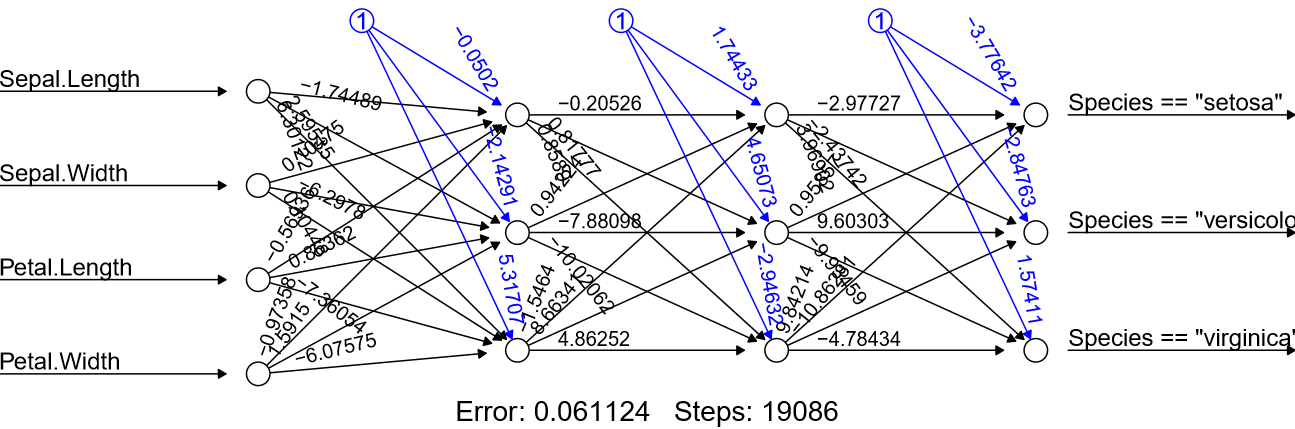
\includegraphics[scale=0.6] {figure/neuralnet_model.png}
\end{figure}
The model visualization allows to see if our model corresponds to the hyperparameters we used during training. However, this is not opitimized for models that use a high number of hidden layers and neurons.\\

Finally, to see our model performance on the test dataset, we can use the \textbf{predict} function.
\begin{knitrout}
\definecolor{shadecolor}{rgb}{0.969, 0.969, 0.969}\color{fgcolor}\begin{kframe}
\begin{alltt}
\hlstd{neuralnet_prediction} \hlkwb{<-} \hlkwd{predict}\hlstd{(neuralnet_model, iris_test)}
\hlkwd{table}\hlstd{(iris_test}\hlopt{$}\hlstd{Species,} \hlkwd{apply}\hlstd{(neuralnet_prediction,} \hlnum{1}\hlstd{, which.max))}
\end{alltt}
\begin{verbatim}
##             
##               1  2  3
##   setosa     14  0  0
##   versicolor  0 17  1
##   virginica   0  0 13
\end{verbatim}
\end{kframe}
\end{knitrout}

The accuracy of this resources is
\begin{knitrout}
\definecolor{shadecolor}{rgb}{0.969, 0.969, 0.969}\color{fgcolor}\begin{kframe}
\begin{verbatim}
## [1] 0.9777778
\end{verbatim}
\end{kframe}
\end{knitrout}
and the time it took to train is :
\begin{knitrout}
\definecolor{shadecolor}{rgb}{0.969, 0.969, 0.969}\color{fgcolor}\begin{kframe}
\begin{verbatim}
## Time difference of 9.78815 secs
\end{verbatim}
\end{kframe}
\end{knitrout}

%%%%%%%%%%%%%%%% Keras %%%%%%%%%%%%%%%% 
\subsection{Keras}
\subsubsection{Installation}
First step, is the installation and download of the Keras files from GitHub :
\begin{knitrout}
\definecolor{shadecolor}{rgb}{0.969, 0.969, 0.969}\color{fgcolor}\begin{kframe}
\begin{alltt}
\hlstd{devtools}\hlopt{::}\hlkwd{install_github}\hlstd{(}\hlstr{"rstudio/keras"}\hlstd{)}
\end{alltt}
\end{kframe}
\end{knitrout}
Then, we need to to install the package and import in the project :
\begin{knitrout}
\definecolor{shadecolor}{rgb}{0.969, 0.969, 0.969}\color{fgcolor}\begin{kframe}
\begin{alltt}
\hlkwd{library}\hlstd{(keras)}
\hlkwd{install_keras}\hlstd{()}
\end{alltt}
\end{kframe}
\end{knitrout}
When the "\textit{Installation complete.}" message appear you have a complete installation with CPU configure on the TensorFlow backend.
If you want to take advantage of your GPU (Ensure that you have the hardware prerequisites) you will need to execute a different command as follows:
\begin{knitrout}
\definecolor{shadecolor}{rgb}{0.969, 0.969, 0.969}\color{fgcolor}\begin{kframe}
\begin{alltt}
\hlkwd{install_keras}\hlstd{(}\hlkwc{tensorflow} \hlstd{=} \hlstr{"gpu"}\hlstd{)}
\end{alltt}
\end{kframe}
\end{knitrout}
\subsubsection{FNN}

First of all we need to load the data and in order to do so we will use the datasets packages. We the data is in the workspace it will be divided into train and test.
\begin{knitrout}
\definecolor{shadecolor}{rgb}{0.969, 0.969, 0.969}\color{fgcolor}\begin{kframe}
\begin{alltt}
\hlkwd{library}\hlstd{(datasets)}
\hlcom{# Download the Iris data to workspace}
\hlkwd{data}\hlstd{(iris)}
\hlcom{# Change the data Iris output for string }
\hlstd{iris}\hlopt{$}\hlstd{Species} \hlkwb{=} \hlkwd{sapply}\hlstd{(}\hlkwd{as.character}\hlstd{(iris}\hlopt{$}\hlstd{Species),}
                      \hlstd{switch,} \hlstr{"setosa"} \hlstd{=} \hlnum{1}\hlstd{,}
                      \hlstr{"versicolor"} \hlstd{=} \hlnum{2}\hlstd{,}
                      \hlstr{"virginica"} \hlstd{=} \hlnum{3}\hlstd{,}
                      \hlkwc{USE.NAMES} \hlstd{= F)}
\hlcom{# Here is another way, to split the data to }
\hlstd{spec} \hlkwb{=} \hlkwd{c}\hlstd{(}\hlkwc{train} \hlstd{=} \hlnum{.7}\hlstd{,}\hlkwc{test} \hlstd{=} \hlnum{.3}\hlstd{)}
\hlcom{# Set a seed in order to be repreductible}
\hlkwd{set.seed}\hlstd{(}\hlnum{123}\hlstd{)}
\hlcom{# Sample through the dataframe using the sample and cut.}
\hlcom{# The variable "g" returns a list of rows for train and}
\hlcom{# test}
\hlstd{g} \hlkwb{=} \hlkwd{sample}\hlstd{(}\hlkwd{cut}\hlstd{(}\hlkwd{seq}\hlstd{(}\hlkwd{nrow}\hlstd{(iris)),}
               \hlkwd{nrow}\hlstd{(iris)}\hlopt{*}\hlkwd{cumsum}\hlstd{(}\hlkwd{c}\hlstd{(}\hlnum{0}\hlstd{,spec)),}
               \hlkwc{labels} \hlstd{=} \hlkwd{names}\hlstd{(spec)}
               \hlstd{)}
           \hlstd{)}
\hlcom{# Use the data and the row information to select rows}
\hlstd{data_df} \hlkwb{=} \hlkwd{split}\hlstd{(iris, g)}
\hlcom{# Create vector that will contain X (Features variable)}
\hlcom{# and Y the target variable}
\hlstd{X} \hlkwb{=} \hlkwd{c}\hlstd{()}
\hlstd{Y} \hlkwb{=} \hlkwd{c}\hlstd{()}
\hlstd{X}\hlopt{$}\hlstd{train} \hlkwb{=} \hlkwd{as.matrix}\hlstd{(data_df}\hlopt{$}\hlstd{train[,}\hlopt{-}\hlkwd{ncol}\hlstd{(data_df}\hlopt{$}\hlstd{train)])}
\hlstd{X}\hlopt{$}\hlstd{test} \hlkwb{=} \hlkwd{as.matrix}\hlstd{(data_df}\hlopt{$}\hlstd{test[,}\hlopt{-}\hlkwd{ncol}\hlstd{(data_df}\hlopt{$}\hlstd{test)])}
\hlstd{Y}\hlopt{$}\hlstd{train} \hlkwb{=} \hlkwd{as.matrix}\hlstd{(data_df}\hlopt{$}\hlstd{train[,}\hlkwd{ncol}\hlstd{(data_df}\hlopt{$}\hlstd{train)])}
\hlstd{Y}\hlopt{$}\hlstd{test} \hlkwb{=} \hlkwd{as.matrix}\hlstd{(data_df}\hlopt{$}\hlstd{test[,}\hlkwd{ncol}\hlstd{(data_df}\hlopt{$}\hlstd{test)],)}
\end{alltt}
\end{kframe}
\end{knitrout}

When the data is ready, it is time to create the FFN. As an analogy, the keras model should be constructed like a Lego toy game. It starts from the input and goes all the way to the output.
\begin{knitrout}
\definecolor{shadecolor}{rgb}{0.969, 0.969, 0.969}\color{fgcolor}\begin{kframe}
\begin{alltt}
\hlcom{# load the library }
\hlkwd{library}\hlstd{(keras)}
\hlcom{# Create a sequential model}
\hlstd{model_keras} \hlkwb{=} \hlkwd{keras_model_sequential}\hlstd{()}
\hlcom{# Start assembling the model with the first layer as the input.}
\hlcom{# A softmax was use in the output because of the }
\hlstd{model_keras} \hlopt
  \hlkwd{layer_dense}\hlstd{(}\hlkwc{units} \hlstd{=} \hlnum{8}\hlstd{,} \hlkwc{activation} \hlstd{=} \hlstr{'relu'}\hlstd{,} \hlkwc{input_shape} \hlstd{=} \hlkwd{c}\hlstd{(}\hlnum{4}\hlstd{))} \hlopt
  \hlkwd{layer_dense}\hlstd{(}\hlkwc{units} \hlstd{=} \hlnum{4}\hlstd{,} \hlkwc{activation} \hlstd{=} \hlstr{'softmax'}\hlstd{)}
\hlcom{# Compile model}
\end{alltt}
\end{kframe}
\end{knitrout}

Here is a quick evaluation of the model created.
\begin{knitrout}
\definecolor{shadecolor}{rgb}{0.969, 0.969, 0.969}\color{fgcolor}\begin{kframe}
\begin{alltt}
\hlkwd{summary}(model_keras)
Model: \hlstr{"sequential"}
________________________________________________________
\hlkwd{Layer} (type)             Output Shape          Param \hlcom{#  }
========================================================
\hlkwd{dense_1} (Dense)          (None, 8)             40       
________________________________________________________
\hlkwd{dense_2} (Dense)          (None, 4)             36       
========================================================
Total params: 76
Trainable params: 76
Non-trainable params: 0
________________________________________________________
\end{alltt}
\end{kframe}
\end{knitrout}

The next steps, is the compilation. In this example, it is important to keep in mind that not all the parameters are use. The loss function, the optimizer and the metrics are the most basic characteristic of an FNN.
\begin{knitrout}
\definecolor{shadecolor}{rgb}{0.969, 0.969, 0.969}\color{fgcolor}\begin{kframe}
\begin{alltt}
\hlstd{model_keras} \hlopt \hlkwd{compile}\hlstd{(}
  \hlkwc{loss} \hlstd{=} \hlstr{'categorical_crossentropy'}\hlstd{,}
  \hlkwc{optimizer} \hlstd{=} \hlkwd{optimizer_adam}\hlstd{(),}
  \hlkwc{metrics} \hlstd{=} \hlkwd{c}\hlstd{(}\hlstr{'accuracy'}\hlstd{)}
\hlstd{)}
\end{alltt}
\end{kframe}
\end{knitrout}

The next step is really important because it is the training part.
\begin{knitrout}
\definecolor{shadecolor}{rgb}{0.969, 0.969, 0.969}\color{fgcolor}\begin{kframe}
\begin{alltt}
\hlstd{history} \hlkwb{<-} \hlstd{model_keras} \hlopt \hlkwd{fit}\hlstd{(}
  \hlkwd{as.matrix}\hlstd{(X}\hlopt{$}\hlstd{train),}\hlkwd{to_categorical}\hlstd{(Y}\hlopt{$}\hlstd{train),}
   \hlkwc{epochs}\hlstd{=}\hlnum{200}\hlstd{,} \hlkwc{batch_size}\hlstd{=}\hlnum{5}\hlstd{)}
\end{alltt}
\end{kframe}
\end{knitrout}

This package of the possibility to store the training history :
\begin{knitrout}
\definecolor{shadecolor}{rgb}{0.969, 0.969, 0.969}\color{fgcolor}\begin{kframe}
\begin{alltt}
\hlkwd{plot}\hlstd{(history)}
\end{alltt}


{\ttfamily\noindent\itshape\color{messagecolor}{\#\# `geom\_smooth()` using formula 'y \textasciitilde{} x'}}\end{kframe}
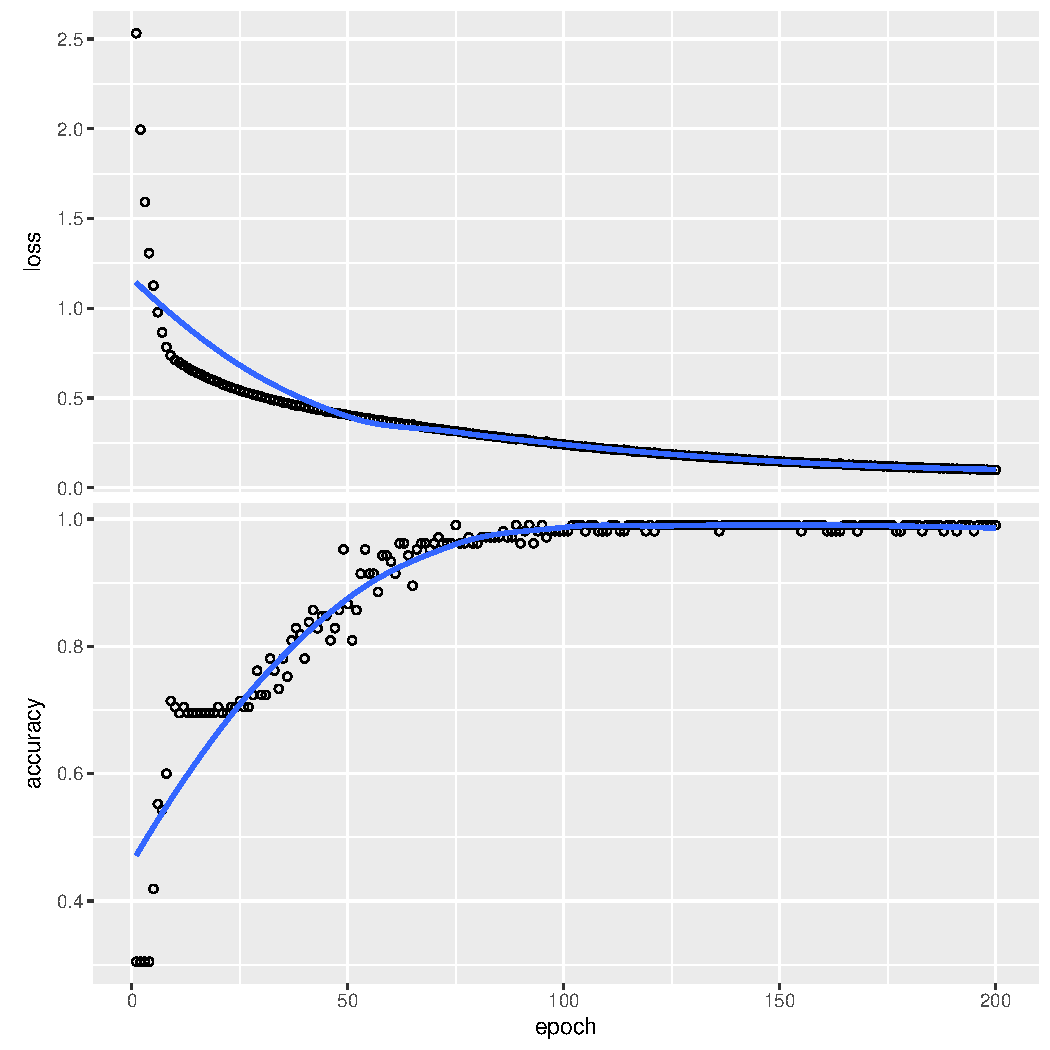
\includegraphics[width=4in]{figure/unnamed-chunk-29-1} 

\end{knitrout}

The final step is just to provide an accuracy of the model.
\begin{knitrout}
\definecolor{shadecolor}{rgb}{0.969, 0.969, 0.969}\color{fgcolor}\begin{kframe}
\begin{alltt}
\hlstd{preds} \hlkwb{=} \hlkwd{predict}\hlstd{(model_keras,}\hlkwd{as.array}\hlstd{(X}\hlopt{$}\hlstd{test))}
\hlstd{pred.label.keras} \hlkwb{<-} \hlkwd{max.col}\hlstd{((preds))} \hlopt{-} \hlnum{1}
\hlnum{1}\hlopt{-}\hlkwd{mean}\hlstd{(pred.label.keras} \hlopt{!=} \hlkwd{as.vector}\hlstd{(data_df}\hlopt{$}\hlstd{test}\hlopt{$}\hlstd{Species))}
\end{alltt}
\end{kframe}
\end{knitrout}


The accuracy of this resources is
\begin{knitrout}
\definecolor{shadecolor}{rgb}{0.969, 0.969, 0.969}\color{fgcolor}\begin{kframe}
\begin{alltt}
[1] 0.9555556
\end{alltt}
\end{kframe}
\end{knitrout}
and the time it took to train is :
\begin{knitrout}
\definecolor{shadecolor}{rgb}{0.969, 0.969, 0.969}\color{fgcolor}\begin{kframe}
\begin{verbatim}
## Time difference of 1.213505 mins
\end{verbatim}
\end{kframe}
\end{knitrout}

\subsubsection{CNN}
The first step consists of loading the CIFAR-10 dataset and creating a train and a test set.
\begin{knitrout}
\definecolor{shadecolor}{rgb}{0.969, 0.969, 0.969}\color{fgcolor}\begin{kframe}
\begin{alltt}
\hlkwd{library}\hlstd{(keras)}
\hlcom{# We set the seed to get all the outputs reproductible.}
\hlkwd{set.seed}\hlstd{(}\hlnum{123}\hlstd{)}
\hlstd{cifar_10} \hlkwb{=} \hlkwd{dataset_cifar10}\hlstd{()}
\hlcom{# RGB values are usually encoded between 0 and 255.}
\hlcom{# A good practice is to scale them to a value from 0 and 1 b dividing the RGB values by 255.}
\hlstd{X_train} \hlkwb{<-} \hlstd{cifar_10}\hlopt{$}\hlstd{train}\hlopt{$}\hlstd{x}\hlopt{/}\hlnum{255}
\hlstd{X_test} \hlkwb{<-} \hlstd{cifar_10}\hlopt{$}\hlstd{test}\hlopt{$}\hlstd{x}\hlopt{/}\hlnum{255}

\hlcom{# cifar_10 class labels ranging from 0 to 9 are downloaded as integer}
\hlcom{# We will use the keras function "to_categorical" to encode them as one-hot.}
\hlstd{Y_train} \hlkwb{<-} \hlkwd{to_categorical}\hlstd{(cifar_10}\hlopt{$}\hlstd{train}\hlopt{$}\hlstd{y,} \hlkwc{num_classes} \hlstd{=} \hlnum{10}\hlstd{)}
\hlstd{Y_test} \hlkwb{<-} \hlkwd{to_categorical}\hlstd{(cifar_10}\hlopt{$}\hlstd{test}\hlopt{$}\hlstd{y,} \hlkwc{num_classes} \hlstd{=} \hlnum{10}\hlstd{)}
\end{alltt}
\end{kframe}
\end{knitrout}
To get an understanding of our data we can plot the 6 first images with a for loop.
\begin{knitrout}
\definecolor{shadecolor}{rgb}{0.969, 0.969, 0.969}\color{fgcolor}\begin{kframe}
\begin{alltt}
\hlkwd{par}\hlstd{(}\hlkwc{mfcol}\hlstd{=}\hlkwd{c}\hlstd{(}\hlnum{2}\hlstd{,}\hlnum{3}\hlstd{))}
\hlkwd{par}\hlstd{(}\hlkwc{mar}\hlstd{=}\hlkwd{c}\hlstd{(}\hlnum{0}\hlstd{,} \hlnum{0}\hlstd{,} \hlnum{1}\hlstd{,} \hlnum{0}\hlstd{),} \hlkwc{xaxs} \hlstd{=} \hlstr{'i'}\hlstd{,} \hlkwc{yaxs}\hlstd{=}\hlstr{'i'}\hlstd{)}
\hlkwa{for} \hlstd{(i} \hlkwa{in} \hlnum{1}\hlopt{:}\hlnum{6}\hlstd{) \{}
  \hlkwd{plot}\hlstd{(}\hlkwd{as.raster}\hlstd{(X_train[i,,,]))}
\hlstd{\}}
\end{alltt}
\end{kframe}
\end{knitrout}
\begin{figure}[h!]
\centering
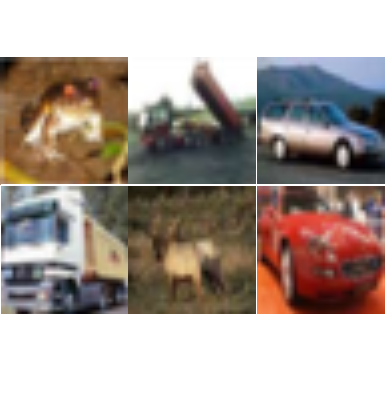
\includegraphics[width=50mm,scale=0.5] {figure/Cifar_10_data_images.png}
\end{figure}
We can now start to implement our CNN model!
\begin{knitrout}
\definecolor{shadecolor}{rgb}{0.969, 0.969, 0.969}\color{fgcolor}\begin{kframe}
\begin{alltt}
\hlcom{# Model implementation}
\hlstd{model} \hlkwb{<-} \hlkwd{keras_model_sequential}\hlstd{()}

\hlstd{model} \hlopt
  \hlcom{# We start with a first 2D convolutional layer, having a kernel of size 3x3.}
  \hlcom{# We use padding = same, meaning that our output tensor will have the same dimensions as our }
  \hlcom{#input tensor.}
  \hlcom{# Our input_shape is the dimension of each of our image. Here we have a 32x32x3 image (RGB).}
  \hlcom{# For black and white images use only 1 dimension (e.g. 32x32x1)}
  \hlkwd{layer_conv_2d}\hlstd{(}\hlkwc{filter} \hlstd{=} \hlnum{32}\hlstd{,} \hlkwc{kernel_size} \hlstd{=} \hlkwd{c}\hlstd{(}\hlnum{3}\hlstd{,}\hlnum{3}\hlstd{),} \hlkwc{padding} \hlstd{=} \hlstr{"same"}\hlstd{,}\hlkwc{input_shape} \hlstd{=} \hlkwd{c}\hlstd{(}\hlnum{32}\hlstd{,} \hlnum{32}\hlstd{,} \hlnum{3}\hlstd{))} \hlopt
  \hlkwd{layer_activation}\hlstd{(}\hlstr{"relu"}\hlstd{)} \hlopt
  \hlkwd{layer_batch_normalization}\hlstd{()} \hlopt

  \hlcom{# We use a 2nd convolutional layer where we increase the number of kernel by 2 (32 -> 64)}
  \hlkwd{layer_conv_2d}\hlstd{(}\hlkwc{filter} \hlstd{=} \hlnum{64}\hlstd{,} \hlkwc{kernel_size} \hlstd{=} \hlkwd{c}\hlstd{(}\hlnum{3}\hlstd{,}\hlnum{3}\hlstd{))} \hlopt
  \hlkwd{layer_activation}\hlstd{(}\hlstr{"relu"}\hlstd{)} \hlopt
  \hlkwd{layer_batch_normalization}\hlstd{()} \hlopt

  \hlcom{# We then use a maxpooling layer in order to reduce the dimentionnality of the }
  \hlcom{#convolutional layer.}
  \hlkwd{layer_max_pooling_2d}\hlstd{(}\hlkwc{pool_size} \hlstd{=} \hlkwd{c}\hlstd{(}\hlnum{2}\hlstd{,}\hlnum{2}\hlstd{))} \hlopt
  \hlkwd{layer_dropout}\hlstd{(}\hlnum{0.25}\hlstd{)} \hlopt

  \hlcom{# We then flatten the maxpooling layer into a vector that will be feed into a FNN.}
  \hlcom{# We set the first layer of our FNN to have 256 hidden neurons.}
  \hlkwd{layer_flatten}\hlstd{()} \hlopt
  \hlkwd{layer_dense}\hlstd{(}\hlnum{256}\hlstd{)} \hlopt
  \hlkwd{layer_activation}\hlstd{(}\hlstr{"relu"}\hlstd{)} \hlopt
  \hlcom{#layer_batch_normalization() %>%}
  \hlkwd{layer_dropout}\hlstd{(}\hlnum{0.5}\hlstd{)} \hlopt

  \hlcom{# We set the output layer of our FNN to have 10 neurons, one for each of the 10 class we }
  \hlcom{#want to predict. We use softmax in order to scale all the output values betwen 0 and 1, }
  \hlcom{#and that the sum of all of them is equal to 1.}
  \hlkwd{layer_dense}\hlstd{(}\hlnum{10}\hlstd{)} \hlopt
  \hlkwd{layer_activation}\hlstd{(}\hlstr{"softmax"}\hlstd{)}
\end{alltt}
\end{kframe}
\end{knitrout}
Our model will have 3,709,002 parameters and can be visualized:
\begin{knitrout}
\definecolor{shadecolor}{rgb}{0.969, 0.969, 0.969}\color{fgcolor}\begin{kframe}
\begin{alltt}
\hlkwd{summary}(model)

Model: \hlstr{"sequential_12"}
______________________________________________________________________________
\hlkwd{Layer} (type)                       Output Shape                   Param \hlcom{#     }
==============================================================================
\hlkwd{conv2d_54} (Conv2D)                 (None, 32, 32, 32)             896         
______________________________________________________________________________
\hlkwd{activation_76} (Activation)         (None, 32, 32, 32)             0           
______________________________________________________________________________
\hlkwd{batch_normalization_52} (\hlkwd{BatchNorma} (None, 32, 32, 32)             128         
______________________________________________________________________________
\hlkwd{conv2d_55} (Conv2D)                 (None, 30, 30, 64)             18496       
______________________________________________________________________________
\hlkwd{activation_77} (Activation)         (None, 30, 30, 64)             0           
______________________________________________________________________________
\hlkwd{batch_normalization_53} (\hlkwd{BatchNorma} (None, 30, 30, 64)             256         
______________________________________________________________________________
\hlkwd{max_pooling2d_26} (MaxPooling2D)    (None, 15, 15, 64)             0           
______________________________________________________________________________
\hlkwd{dropout_38} (Dropout)               (None, 15, 15, 64)             0           
______________________________________________________________________________
\hlkwd{flatten_12} (Flatten)               (None, 14400)                  0           
______________________________________________________________________________
\hlkwd{dense_24} (Dense)                   (None, 256)                    3686656     
______________________________________________________________________________
\hlkwd{activation_78} (Activation)         (None, 256)                    0           
______________________________________________________________________________
\hlkwd{dropout_39} (Dropout)               (None, 256)                    0           
______________________________________________________________________________
\hlkwd{dense_25} (Dense)                   (None, 10)                     2570        
______________________________________________________________________________
\hlkwd{activation_79} (Activation)         (None, 10)                     0           
==============================================================================
Total params: 3,709,002
Trainable params: 3,708,810
Non-trainable params: 192
______________________________________________________________________________
\end{alltt}
\end{kframe}
\end{knitrout}

We then set our hyperparameters to use RMSprop as the optimizater with a learning rate of 1e-3 and a decay of 1e-6. We set our batch size to 64 to use train our model with 64 images per iteration. We set epoch to 10, our model will go trough the entire training set 5 times. 20\% of the training set will be used as validation set, in order to tune the parameters without biais.
\begin{knitrout}
\definecolor{shadecolor}{rgb}{0.969, 0.969, 0.969}\color{fgcolor}\begin{kframe}
\begin{alltt}
\hlstd{opt} \hlkwb{<-} \hlkwd{optimizer_rmsprop}\hlstd{(}\hlkwc{lr} \hlstd{=} \hlnum{1e-3}\hlstd{,} \hlkwc{decay} \hlstd{=} \hlnum{1e-6}\hlstd{)}

\hlstd{batch_size} \hlkwb{<-} \hlnum{64}
\hlstd{epochs} \hlkwb{<-} \hlnum{5}
\hlstd{validation} \hlkwb{<-} \hlnum{0.2}
\end{alltt}
\end{kframe}
\end{knitrout}
We will us as loss function the categorical\_crossentropy that works very well with our softmax activaction function in order to peform multi label classification. We will look at the accuracy as the final metric to check the performance of our model on the test dataset.
\begin{knitrout}
\definecolor{shadecolor}{rgb}{0.969, 0.969, 0.969}\color{fgcolor}\begin{kframe}
\begin{alltt}
\hlstd{model} \hlopt
    \hlkwd{compile}\hlstd{(}\hlkwc{loss} \hlstd{=} \hlstr{"categorical_crossentropy"}\hlstd{,}
            \hlkwc{optimizer} \hlstd{= opt,} \hlkwc{metrics} \hlstd{=} \hlstr{"accuracy"}\hlstd{)}
\end{alltt}
\end{kframe}
\end{knitrout}
Now, we will train our model, and we will store it into a list called \textbf{history}. 
\begin{knitrout}
\definecolor{shadecolor}{rgb}{0.969, 0.969, 0.969}\color{fgcolor}\begin{kframe}
\begin{alltt}
\hlstd{start_time} \hlkwb{<-} \hlkwd{Sys.time}\hlstd{()}
\hlstd{history_cnn_keras} \hlkwb{<-} \hlstd{model} \hlopt \hlkwd{fit}\hlstd{(}
    \hlstd{X_train, Y_train,}
    \hlkwc{batch_size} \hlstd{= batch_size,}
    \hlkwc{epochs} \hlstd{= epochs,}
    \hlkwc{validation_split} \hlstd{= validation,}
    \hlkwc{shuffle} \hlstd{=} \hlnum{TRUE}\hlstd{)}
\hlstd{end_time} \hlkwb{<-} \hlkwd{Sys.time}\hlstd{()}
\hlstd{time_cnn_keras} \hlkwb{=} \hlstd{end_time} \hlopt{-} \hlstd{start_time}
\end{alltt}
\end{kframe}
\end{knitrout}
By default keras plot our model loss and accuracy per epoch on the training set and on the validation set.\\

\begin{figure}[h!]
\centering
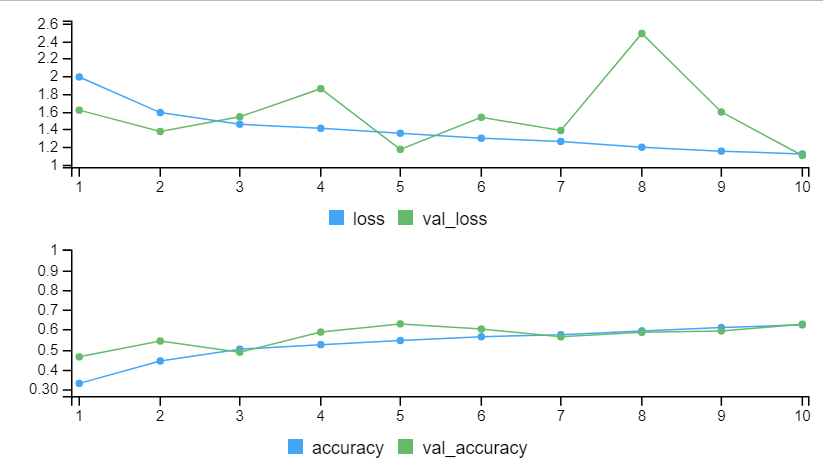
\includegraphics[width=\textwidth]{figure/CNN_keras_graph.png}
\end{figure}
Then, we will evaluate our model performance on our test set.
\begin{knitrout}
\definecolor{shadecolor}{rgb}{0.969, 0.969, 0.969}\color{fgcolor}\begin{kframe}
\begin{alltt}
model %>% \hlkwd{evaluate}(X_test, Y_test,verbose = 0)

$loss
[1] 1.70912

$accuracy
[1] 0.598
\end{alltt}
\end{kframe}
\end{knitrout}
We can see that our accuracy is 59.8\%.\\
And the time it took to train is:
\begin{knitrout}
\definecolor{shadecolor}{rgb}{0.969, 0.969, 0.969}\color{fgcolor}\begin{kframe}
\begin{alltt}
model %>% \hlkwd{evaluate}(X_test, Y_test,verbose = 0)
Time difference of 19.25289 mins
\end{alltt}
\end{kframe}
\end{knitrout}

In order to predict with our model on a new dataset, we can you Keras\'s \textbf{predict\_classes} function.
\begin{knitrout}
\definecolor{shadecolor}{rgb}{0.969, 0.969, 0.969}\color{fgcolor}\begin{kframe}
\begin{alltt}
\hlstd{Y_predicted} \hlkwb{<-} \hlstd{model} \hlopt \hlkwd{predict_classes}\hlstd{(X_test)}
\end{alltt}
\end{kframe}
\end{knitrout}

\subsubsection{RNN}


This is an example that the keras package uses for text classification. However it is not an RNN or in this case an LSTM algorithm.

As a first step it is important to download the data from keras.
\begin{knitrout}
\definecolor{shadecolor}{rgb}{0.969, 0.969, 0.969}\color{fgcolor}\begin{kframe}
\begin{alltt}
\hlkwd{library}\hlstd{(keras)}
\hlkwd{library}\hlstd{(dplyr)}
\hlkwd{library}\hlstd{(ggplot2)}
\hlkwd{library}\hlstd{(purrr)}
\hlstd{word_index} \hlkwb{<-} \hlkwd{dataset_imdb_word_index}\hlstd{()}
\hlkwd{length}\hlstd{(word_index)}
\hlcom{# This is in order to limit the number of words }
\hlstd{max_features} \hlkwb{=} \hlkwd{length}\hlstd{(word_index)}

\hlcom{# cut texts after this number of words (among top max_features most common words)}
\hlstd{maxlen} \hlkwb{=} \hlnum{45}
\end{alltt}
\end{kframe}
\end{knitrout}
Unfortunately, not everything is perfect with the package and some bugs can be found such as this one. The function \textit{dataset\_imdb()} normally returns the dataset with some filter that we pass as parameter. However, the bug\cite{bugRNNkeras} found doing this tutorial is that when the parameter maxlen is less than 150 it returns a null for the test data.
\begin{knitrout}
\definecolor{shadecolor}{rgb}{0.969, 0.969, 0.969}\color{fgcolor}\begin{kframe}
\begin{alltt}
\hlcom{# Loads the dataset which is already split in train and test}
\hlcom{# For some reason there is a bug. When adding the parameter Max len the function don't}
\hlcom{# return test data if not above maxlen 180 }
\hlstd{imdb} \hlkwb{<-} \hlkwd{dataset_imdb}\hlstd{(}\hlkwc{maxlen} \hlstd{= maxlen,} \hlkwc{seed} \hlstd{=} \hlnum{123} \hlstd{)}
\hlstd{imdb_hack} \hlkwb{<-} \hlkwd{dataset_imdb}\hlstd{(}\hlkwc{maxlen} \hlstd{=} \hlnum{180} \hlstd{,} \hlkwc{seed} \hlstd{=} \hlnum{123}\hlstd{)}
\hlstd{imdb}\hlopt{$}\hlstd{train}
\hlstd{imdb_hack}\hlopt{$}\hlstd{test}
\hlcom{# Seperate the labels and the data for train and test}
\hlkwd{c}\hlstd{(train_data, train_labels)} \hlopt \hlstd{imdb}\hlopt{$}\hlstd{train}
\hlkwd{c}\hlstd{(test_data, test_labels)} \hlopt \hlstd{imdb_hack}\hlopt{$}\hlstd{test}

\hlcom{# This is the word index which can be interprate as a dictionnary betweend index to words}
\hlcom{# (e.g.) the word "modestly" is represented by the index 20608}
\hlcom{# by default this word to index contains 88584 words}
\hlstd{max_features}
\hlcom{# Convert this word to index List to a more friendly data frame}
\hlstd{word_index_df} \hlkwb{<-} \hlkwd{data.frame}\hlstd{(}
  \hlkwc{word} \hlstd{=} \hlkwd{names}\hlstd{(word_index),}
  \hlkwc{idx} \hlstd{=} \hlkwd{unlist}\hlstd{(word_index,} \hlkwc{use.names} \hlstd{=} \hlnum{FALSE}\hlstd{),}
  \hlkwc{stringsAsFactors} \hlstd{=} \hlnum{FALSE}
\hlstd{)}

\hlcom{# The first 4 indices are reserved for 4 different specials keys}
\hlcom{# PAD:    This is to fill a sequence that is shorter than Max lenght}
\hlcom{# START:  This is to fill a sequence that is shorter than Max lenght}
\hlcom{# PAD:    This is to fill a sequence that is shorter than Max lenght}
\hlcom{# UNK:    This if for an unkown words that are not part of vocabulary}
\hlcom{# UNUSED: This if for an unused word part of the vocabulary}

\hlstd{word_index_df} \hlkwb{<-} \hlstd{word_index_df} \hlopt \hlkwd{mutate}\hlstd{(}\hlkwc{idx} \hlstd{= idx} \hlopt{+} \hlnum{3}\hlstd{)}
\hlstd{word_index_df} \hlkwb{<-} \hlstd{word_index_df} \hlopt
  \hlkwd{add_row}\hlstd{(}\hlkwc{word} \hlstd{=} \hlstr{"<PAD>"}\hlstd{,} \hlkwc{idx} \hlstd{=} \hlnum{0}\hlstd{)}\hlopt
  \hlkwd{add_row}\hlstd{(}\hlkwc{word} \hlstd{=} \hlstr{"<START>"}\hlstd{,} \hlkwc{idx} \hlstd{=} \hlnum{1}\hlstd{)}\hlopt
  \hlkwd{add_row}\hlstd{(}\hlkwc{word} \hlstd{=} \hlstr{"<UNK>"}\hlstd{,} \hlkwc{idx} \hlstd{=} \hlnum{2}\hlstd{)}\hlopt
  \hlkwd{add_row}\hlstd{(}\hlkwc{word} \hlstd{=} \hlstr{"<UNUSED>"}\hlstd{,} \hlkwc{idx} \hlstd{=} \hlnum{3}\hlstd{)}
\hlcom{# Sort the rows by index}
\hlstd{word_index_df} \hlkwb{<-} \hlstd{word_index_df} \hlopt \hlkwd{arrange}\hlstd{(idx)}
\hlcom{# A function that will decode a id an return the full review}
\hlstd{decode_review} \hlkwb{<-} \hlkwa{function}\hlstd{(}\hlkwc{text}\hlstd{)\{}
  \hlkwd{paste}\hlstd{(}\hlkwd{map}\hlstd{(text,} \hlkwa{function}\hlstd{(}\hlkwc{number}\hlstd{) word_index_df} \hlopt
              \hlkwd{filter}\hlstd{(idx} \hlopt{==} \hlstd{number)} \hlopt
              \hlkwd{select}\hlstd{(word)} \hlopt
              \hlkwd{pull}\hlstd{()),}
        \hlkwc{collapse} \hlstd{=} \hlstr{" "}\hlstd{)}
\hlstd{\}}
\end{alltt}
\end{kframe}
\end{knitrout}


\begin{knitrout}
\definecolor{shadecolor}{rgb}{0.969, 0.969, 0.969}\color{fgcolor}\begin{kframe}
\begin{alltt}
\hlkwd{decode_review}(train_data[[5]])
[1] "<START> excellent episode movie ala pulp fiction 7 days 7 suicides it doesnt get more
depressing than this movie rating 8 10 music rating 10 10"
\end{alltt}
\end{kframe}
\end{knitrout}

\begin{knitrout}
\definecolor{shadecolor}{rgb}{0.969, 0.969, 0.969}\color{fgcolor}\begin{kframe}
\begin{alltt}
\hlcom{# This function is built in the Keras environmet and as the name indicates it}
\hlcom{# is use for padding sequences such as our reviews. after this is done all the}
\hlcom{# review will have the same lenght. The shorter ones will be filled with the token}
\hlcom{# <pad>. This applies to the train and test data.}
\hlstd{train_pad} \hlkwb{<-} \hlkwd{pad_sequences}\hlstd{(}
  \hlstd{train_data,}
  \hlkwc{value} \hlstd{= word_index_df} \hlopt \hlkwd{filter}\hlstd{(word} \hlopt{==} \hlstr{"<PAD>"}\hlstd{)} \hlopt \hlkwd{select}\hlstd{(idx)} \hlopt \hlkwd{pull}\hlstd{(),}
  \hlkwc{padding} \hlstd{=} \hlstr{"post"}\hlstd{,}
  \hlkwc{maxlen} \hlstd{= maxlen}
\hlstd{)}

\hlstd{test_pad} \hlkwb{<-} \hlkwd{pad_sequences}\hlstd{(}
  \hlstd{test_data,}
  \hlkwc{value} \hlstd{= word_index_df} \hlopt \hlkwd{filter}\hlstd{(word} \hlopt{==} \hlstr{"<PAD>"}\hlstd{)} \hlopt \hlkwd{select}\hlstd{(idx)} \hlopt \hlkwd{pull}\hlstd{(),}
  \hlkwc{padding} \hlstd{=} \hlstr{"post"}\hlstd{,}
  \hlkwc{maxlen} \hlstd{= maxlen}
\hlstd{)}


\hlstd{model} \hlkwb{<-} \hlkwd{keras_model_sequential}\hlstd{()}
\hlstd{model} \hlopt
  \hlkwd{layer_embedding}\hlstd{(}\hlkwc{input_dim} \hlstd{= max_features,} \hlkwc{output_dim} \hlstd{=} \hlnum{32}\hlstd{)} \hlopt
  \hlkwd{layer_lstm}\hlstd{(}\hlkwc{units} \hlstd{=} \hlnum{24}\hlstd{,}
             \hlkwc{input_shape} \hlstd{=} \hlnum{32}\hlstd{,}
             \hlkwc{batch_size} \hlstd{=} \hlnum{8}\hlstd{)}\hlopt
  \hlkwd{layer_dropout}\hlstd{(}\hlkwc{rate} \hlstd{=} \hlnum{0.1}\hlstd{)} \hlopt
  \hlkwd{layer_dense}\hlstd{(}\hlkwc{units} \hlstd{=} \hlnum{1}\hlstd{,} \hlkwc{activation} \hlstd{=} \hlstr{"relu"}\hlstd{)}

\hlstd{model} \hlopt \hlkwd{summary}\hlstd{()}

\hlstd{model} \hlopt \hlkwd{compile}\hlstd{(}
  \hlkwc{optimizer} \hlstd{=} \hlstr{'adam'}\hlstd{,}
  \hlkwc{loss} \hlstd{=} \hlstr{'binary_crossentropy'}\hlstd{,}
  \hlkwc{metrics} \hlstd{=} \hlkwd{list}\hlstd{(}\hlstr{'accuracy'}\hlstd{)}
\hlstd{)}


\hlcom{#Create a validation dataset}
\hlstd{n} \hlkwb{=} \hlkwd{as.integer}\hlstd{(}\hlkwd{round}\hlstd{(}\hlkwd{nrow}\hlstd{(train_pad)}\hlopt{*}\hlnum{0.7}\hlstd{))}
\hlstd{x_val} \hlkwb{<-} \hlstd{train_pad[}\hlnum{1}\hlopt{:}\hlstd{n, ]}
\hlstd{partial_x_train} \hlkwb{<-} \hlstd{train_pad[(n}\hlopt{+}\hlnum{1}\hlstd{)}\hlopt{:}\hlkwd{nrow}\hlstd{(train_pad), ]}

\hlstd{y_val} \hlkwb{<-} \hlstd{train_labels[}\hlnum{1}\hlopt{:}\hlstd{n]}
\hlstd{partial_y_train} \hlkwb{<-} \hlstd{train_labels[(n}\hlopt{+}\hlnum{1}\hlstd{)}\hlopt{:}\hlkwd{length}\hlstd{(train_labels)]}


\hlstd{start_time} \hlkwb{<-} \hlkwd{Sys.time}\hlstd{()}
\hlstd{history_rnn_keras} \hlkwb{<-} \hlstd{model} \hlopt \hlkwd{fit}\hlstd{(}
  \hlstd{partial_x_train,}
  \hlstd{partial_y_train,}
  \hlkwc{epochs} \hlstd{=} \hlnum{20}\hlstd{,}
  \hlkwc{validation_data} \hlstd{=} \hlkwd{list}\hlstd{(x_val, y_val),}
\hlstd{)}
\hlstd{end_time} \hlkwb{<-} \hlkwd{Sys.time}\hlstd{()}
\hlstd{time_rnn_keras} \hlkwb{=} \hlstd{end_time} \hlopt{-} \hlstd{start_time}

\hlstd{results} \hlkwb{<-} \hlstd{model} \hlopt \hlkwd{evaluate}\hlstd{(test_pad, test_labels)}
\end{alltt}
\end{kframe}
\end{knitrout}
The training history can be plot by calling the history :
\begin{knitrout}
\definecolor{shadecolor}{rgb}{0.969, 0.969, 0.969}\color{fgcolor}\begin{kframe}
\begin{alltt}
\hlkwd{plot}\hlstd{(history_rnn_keras)}
\end{alltt}


{\ttfamily\noindent\itshape\color{messagecolor}{\#\# `geom\_smooth()` using formula 'y \textasciitilde{} x'}}\end{kframe}
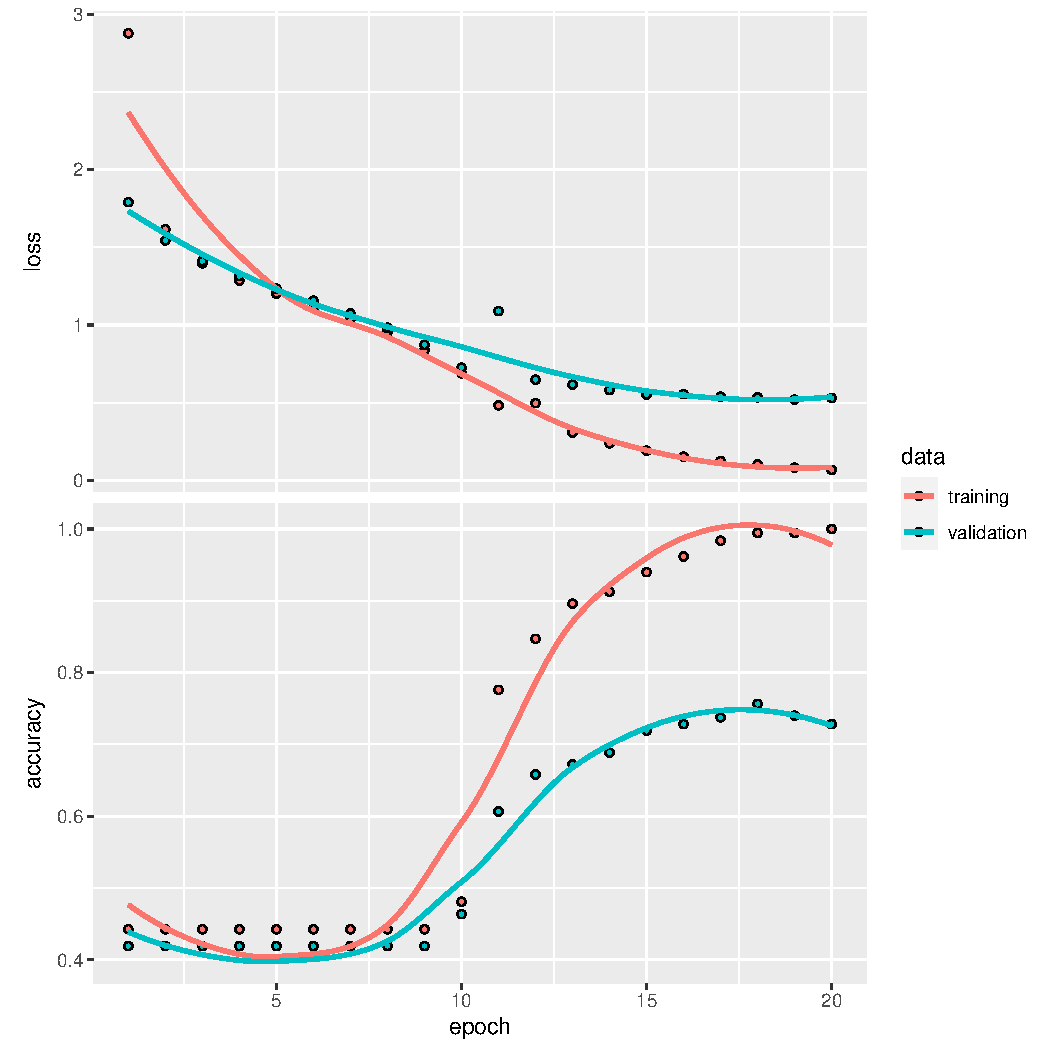
\includegraphics[width=6in]{figure/unnamed-chunk-49-1} 

\end{knitrout}
The accuracy of the model is as follow :
\begin{knitrout}
\definecolor{shadecolor}{rgb}{0.969, 0.969, 0.969}\color{fgcolor}\begin{kframe}
\begin{alltt}
\hlstd{results}
\end{alltt}
\begin{verbatim}
## $loss
## [1] 0.6962709
## 
## $accuracy
## [1] 0.6293246
\end{verbatim}
\end{kframe}
\end{knitrout}
%%%%%%%%%%%%%%%% H2o %%%%%%%%%%%%%%%% 
\subsection{h2o}
\subsubsection{Installation}
\begin{knitrout}
\definecolor{shadecolor}{rgb}{0.969, 0.969, 0.969}\color{fgcolor}\begin{kframe}
\begin{alltt}
\hlkwd{install.packages}\hlstd{(}\hlstr{"h2o"}\hlstd{)}
\hlkwd{library}\hlstd{(h2o)}
\hlkwd{h2o.init}\hlstd{()}
\end{alltt}
\end{kframe}
\end{knitrout}
By default, H2O Deep Learning uses an adaptive learning rate (ADADELTA) for its stochastic gradient descent optimization.
\textbf{Prerequisites to launch H2o}, 64 bit Java 6+ if you want to open a h2o model that s more than 1 GB. 
\subsubsection{FNN}
\begin{knitrout}
\definecolor{shadecolor}{rgb}{0.969, 0.969, 0.969}\color{fgcolor}\begin{kframe}
\begin{alltt}
\hlkwd{library}\hlstd{(h2o)}
\hlkwd{h2o.init}\hlstd{()}
\hlcom{# Identify predictors and response}


\hlstd{h2o_df_train} \hlkwb{=} \hlkwd{as.h2o}\hlstd{(data_df}\hlopt{$}\hlstd{train)}
\hlstd{h2o_df_test} \hlkwb{=} \hlkwd{as.h2o}\hlstd{(data_df}\hlopt{$}\hlstd{test)}

\hlstd{y} \hlkwb{<-} \hlstr{"Species"}
\hlstd{x} \hlkwb{<-} \hlkwd{setdiff}\hlstd{(}\hlkwd{names}\hlstd{(h2o_df_train), y)}
\hlcom{# For binary classification, response should be a factor}
\hlstd{h2o_df_train[,y]} \hlkwb{<-} \hlkwd{as.factor}\hlstd{(h2o_df_train[,y])}
\hlstd{h2o_df_test[,y]} \hlkwb{<-} \hlkwd{as.factor}\hlstd{(h2o_df_test[,y])}

\hlstd{start_time} \hlkwb{<-} \hlkwd{Sys.time}\hlstd{()}
\hlstd{model_h2o} \hlkwb{<-} \hlkwd{h2o.deeplearning}\hlstd{(}\hlkwc{x} \hlstd{= x,}
                              \hlkwc{y} \hlstd{= y,}
                              \hlkwc{training_frame} \hlstd{= h2o_df_train,}
                              \hlkwc{epochs} \hlstd{=} \hlnum{200}\hlstd{,}
                              \hlkwc{seed}\hlstd{=}\hlnum{123}\hlstd{)}
\hlstd{end_time} \hlkwb{<-} \hlkwd{Sys.time}\hlstd{()}
\hlstd{time_fnn_h2o} \hlkwb{=} \hlstd{end_time} \hlopt{-} \hlstd{start_time}

\hlkwd{summary}\hlstd{(model_h2o)}

\hlstd{perf} \hlkwb{<-} \hlkwd{h2o.performance}\hlstd{(model_h2o,} \hlkwd{as.h2o}\hlstd{(data_df}\hlopt{$}\hlstd{test))}
\hlstd{pred} \hlkwb{<-} \hlkwd{h2o.predict}\hlstd{(model_h2o,} \hlkwd{as.h2o}\hlstd{(data_df}\hlopt{$}\hlstd{test))}
\hlnum{1}\hlopt{-}\hlkwd{mean}\hlstd{(}\hlkwd{as.vector}\hlstd{(pred}\hlopt{$}\hlstd{predict)} \hlopt{!=} \hlkwd{as.vector}\hlstd{(data_df}\hlopt{$}\hlstd{test}\hlopt{$}\hlstd{Species))}
\end{alltt}
\end{kframe}
\end{knitrout}
The accuracy of this resources is
\begin{knitrout}
\definecolor{shadecolor}{rgb}{0.969, 0.969, 0.969}\color{fgcolor}\begin{kframe}
\begin{verbatim}
## [1] 0.9333333
\end{verbatim}
\end{kframe}
\end{knitrout}
and the time it took to train is :
\begin{knitrout}
\definecolor{shadecolor}{rgb}{0.969, 0.969, 0.969}\color{fgcolor}\begin{kframe}
\begin{verbatim}
## Time difference of 7.731083 secs
\end{verbatim}
\end{kframe}
\end{knitrout}
\subsubsection{CNN}
\subsubsection{RNN}


%%%%%%%%%%%%%%%% MXNET %%%%%%%%%%%%%%%% 
\subsection{MXNET}
\subsubsection{Installation}
For CPU :
\begin{knitrout}
\definecolor{shadecolor}{rgb}{0.969, 0.969, 0.969}\color{fgcolor}\begin{kframe}
\begin{alltt}
\hlkwd{install.packages}\hlstd{(}\hlstr{"https://s3.ca-central-1.amazonaws.com/jeremiedb/share/mxnet/CPU/mxnet.zip"}\hlstd{,}
                 \hlkwc{repos} \hlstd{=} \hlkwa{NULL}\hlstd{)}
\hlkwd{library}\hlstd{(mxnet)}
\end{alltt}
\end{kframe}
\end{knitrout}

\subsubsection{FNN}
\begin{knitrout}
\definecolor{shadecolor}{rgb}{0.969, 0.969, 0.969}\color{fgcolor}\begin{kframe}
\begin{alltt}
\hlkwd{install.packages}\hlstd{(}\hlstr{"https://s3.ca-central-1.amazonaws.com/jeremiedb/share/mxnet/CPU/mxnet.zip"}\hlstd{,} \hlkwc{repos} \hlstd{=} \hlkwa{NULL}\hlstd{)}
\hlkwd{library}\hlstd{(mxnet)}
\hlstd{data} \hlkwb{<-} \hlkwd{mx.symbol.Variable}\hlstd{(}\hlstr{"data"}\hlstd{)}
\hlstd{fc1} \hlkwb{<-} \hlkwd{mx.symbol.FullyConnected}\hlstd{(data,} \hlkwc{name}\hlstd{=}\hlstr{"fc1"}\hlstd{,} \hlkwc{num_hidden}\hlstd{=}\hlnum{8}\hlstd{)}
\hlstd{act1} \hlkwb{<-} \hlkwd{mx.symbol.Activation}\hlstd{(fc1,} \hlkwc{name}\hlstd{=}\hlstr{"relu1"}\hlstd{,} \hlkwc{act_type}\hlstd{=}\hlstr{"relu"}\hlstd{)}
\hlstd{fc2} \hlkwb{<-} \hlkwd{mx.symbol.FullyConnected}\hlstd{(act1,} \hlkwc{name}\hlstd{=}\hlstr{"fc2"}\hlstd{,} \hlkwc{num_hidden}\hlstd{=}\hlnum{3}\hlstd{)}
\hlstd{softmax} \hlkwb{<-} \hlkwd{mx.symbol.SoftmaxOutput}\hlstd{(fc2,} \hlkwc{name}\hlstd{=}\hlstr{"sm"}\hlstd{)}
\hlkwd{mx.set.seed}\hlstd{(}\hlnum{123}\hlstd{)}

\hlstd{start_time} \hlkwb{<-} \hlkwd{Sys.time}\hlstd{()}
\hlstd{model_mx} \hlkwb{<-} \hlkwd{mx.model.FeedForward.create}\hlstd{(}
  \hlstd{softmax,}
  \hlkwc{X}\hlstd{=}\hlkwd{as.array}\hlstd{(X}\hlopt{$}\hlstd{train),}
  \hlkwc{y}\hlstd{=}\hlkwd{as.numeric}\hlstd{(Y}\hlopt{$}\hlstd{train),}
  \hlkwc{ctx}\hlstd{=}\hlkwd{mx.cpu}\hlstd{(),}
  \hlkwc{num.round}\hlstd{=}\hlnum{200}\hlstd{,}
  \hlkwc{verbose} \hlstd{=} \hlnum{TRUE}\hlstd{,}
  \hlkwc{eval.metric} \hlstd{= mx.metric.accuracy,}
  \hlkwc{array.batch.size}\hlstd{=}\hlnum{5}\hlstd{)}
\hlstd{end_time} \hlkwb{<-} \hlkwd{Sys.time}\hlstd{()}
\hlstd{time_fnn_mxnet} \hlkwb{=} \hlstd{end_time} \hlopt{-} \hlstd{start_time}


\hlstd{preds} \hlkwb{=} \hlkwd{predict}\hlstd{(model_mx,}\hlkwd{as.array}\hlstd{(X}\hlopt{$}\hlstd{test),}\hlkwc{array.layout} \hlstd{=} \hlstr{"rowmajor"}\hlstd{)}
\hlkwd{summary}\hlstd{(model_mx)}
\hlstd{pred.label.mxnet} \hlkwb{<-} \hlkwd{max.col}\hlstd{(}\hlkwd{t}\hlstd{(preds))} \hlopt{-} \hlnum{1}
\hlnum{1}\hlopt{-}\hlkwd{mean}\hlstd{(pred.label.mxnet} \hlopt{!=} \hlkwd{as.vector}\hlstd{(data_df}\hlopt{$}\hlstd{test}\hlopt{$}\hlstd{Species))}
\end{alltt}
\end{kframe}
\end{knitrout}
The accuracy of this resources is
\begin{knitrout}
\definecolor{shadecolor}{rgb}{0.969, 0.969, 0.969}\color{fgcolor}\begin{kframe}
\begin{verbatim}
## [1] 0.9333333
\end{verbatim}
\end{kframe}
\end{knitrout}
and the time it took to train is :
\begin{knitrout}
\definecolor{shadecolor}{rgb}{0.969, 0.969, 0.969}\color{fgcolor}\begin{kframe}
\begin{verbatim}
## Time difference of 6.597001 secs
\end{verbatim}
\end{kframe}
\end{knitrout}


%%%%%%%%%%%%%%%%%%%%%%%%%%%%%%%%%%%%%%%%%%%%%%%%%%%
%%%%%%%%%%%%%%%%%% Discussion  %%%%%%%%%%%%%%%%%%%%
%%%%%%%%%%%%%%%%%%%%%%%%%%%%%%%%%%%%%%%%%%%%%%%%%%%
\section{Discussion}
\subsection{FNN}
The CRAN platform includes a lot of packages allowing to use different types of FNN, going from one hidden layers FNN to deep FNN. Vanilla FNN and deep FNN can be easily implemented and plotted with the package \textbf{neuralnet}, while more advanced architecture such as bayesian regularized neural networks are available with the package \textbf{brnn}. If you decide to use one of the package available on CRAN, we highly recommend to read the package documentation, as default parameters, backpropagation algorthms, activation functions may vary from one package to another. However, for building deep FNN in R, we highly suggest to use Keras API, as it will give you much more flexibility and will allow you to use the latest deep FNN architectures. Keras has a lot of advantages such as building your model layer by layer and using different types of hidden activation functions such as Relu, and different output activation functions such as softmax. However, we discovered some bugs while using Keras, especially while downloading datasets and we recommend therefore to carefully check your data at each step of the model construction.
\subsection{CNN}
\subsection{RNN}

%%%%%%%%%%%%%%%%%%%%%%%%%%%%%%%%%%%%%%%%%%%%%%%%%%%
%%%%%%%%%%%%%%%%%% Biblio      %%%%%%%%%%%%%%%%%%%%
%%%%%%%%%%%%%%%%%%%%%%%%%%%%%%%%%%%%%%%%%%%%%%%%%%%
\newpage
\pagestyle{plain}
\bibliography{global.bib}
\end{document}
